\section{Introduction}

This chapter introduces the three open innovation cases recruited for this study. We begin with an overview of each case before comparing these in terms of the number of participants, their demographic and psychological attributes, spatial proximity to one another, knowledge sharing ties, and broker roles. All three cases are quite different, and by the end of this chapter, the reader ought to have a good understanding of each. Without this understanding, it will be harder for the reader to make sense of the results from the exponential random graph modelling and analysis of semi-structured interviews presented in Chapters 6 and 7, respectively. \medskip

\begin{sidewaystable}[p]
\centering
\resizebox{0.9\textwidth}{!}{%	
\begin{threeparttable}
\footnotesize
\setlength{\tabcolsep}{6pt}
\renewcommand{\arraystretch}{1}
\caption[Distinguishing  features of the three open innovation cases]{Distinguishing features of the three open innovation cases.}
\label{tab:cases}
\begin{tabular}{@{}cllccccc@{}}
\toprule
Case & \multicolumn{1}{c}{Description} & \multicolumn{1}{c}{Challenge} & \makecell[tc]{Type of \\Open \\Innovation} & Stage & \makecell[tc]{Partner \\organisations} & \makecell[tc]{Identified \\participants} & 
\makecell[tc]{Actual \\participants}\\ \midrule
1 & Cold-chain innovation & \makecell[tl]{Extend shelf-life of green \\leaf vegetables} & Inbound & Early & 7 & 18 & 18\\
2 & Farm system innovation & \makecell[tl]{Implement a robotic \\dairy based on voluntary \\cow traffic} & Coupled & Closing & 8 & 25 & 25 \\
3 & \makecell[tl]{Global honeybee \\research partnership} & \makecell[tl]{Develop a cloud-based data \\analysis system to track \\honeybee movements in and \\out of hives} & Outbound & Very early & 15 & 45 & 40 \\ \bottomrule
\end{tabular}%
\end{threeparttable}
%
}
\end{sidewaystable}

\section{Case overviews}

The distinguishing features of each case are listed in Table \ref{tab:cases}. We are dealing with a small number of individual participants in each case. Two of the cases were at an early stage of execution, while the third was in its closing stage at the time of data collection. Note that partner names have been altered in the case overviews to protect their identity and the geographic markets in which they operate. 

\begin{sidewaysfigure}
\centering
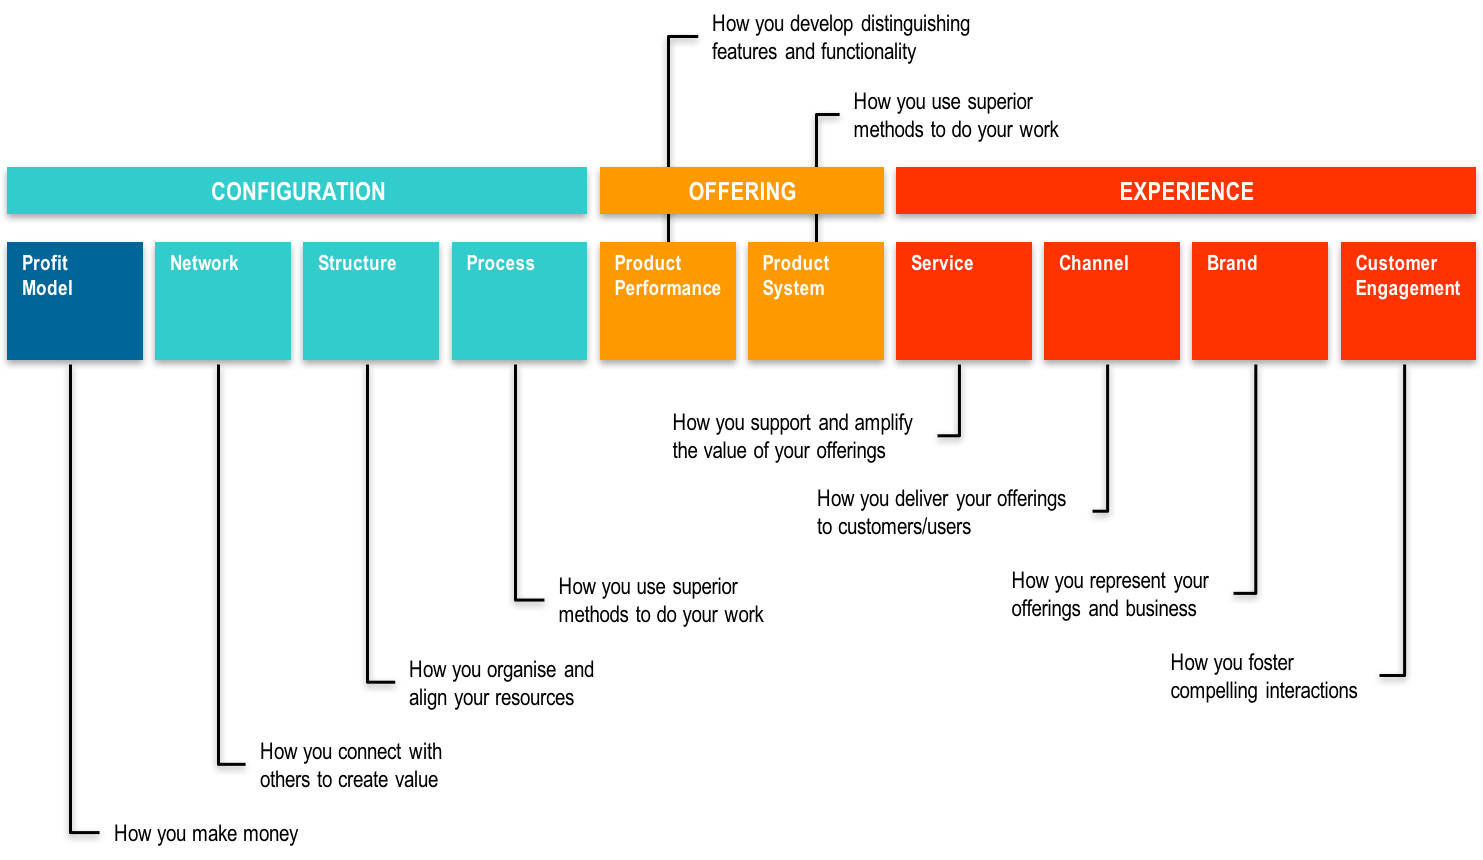
\includegraphics[width = \textwidth]{Images/innovation_types.png}
\caption{Different types of innovation. After \citet{keeley2013ten}.}
\label{fig:innov_type}
\end{sidewaysfigure}

\subsection{Case 1: Cold-chain innovation}

Case 1 revolves around a family-owned business that grows and supplies a range of green leafy vegetable products to caterers, restaurants, local greengrocers, and supermarket chains. Products are supplied either in bulk or in pre-packaged bags sold by the carton. Pre-packaged bags are supplied either as their own branded product or as a supermarket private-label product. The business operates in a region that enjoys a temperate climate, enabling them to grow a greater variety of green leafy vegetables all year round. The business competes with a handful of other firms for supply contracts with national supermarket chains. It views itself as a progressive enterprise that combines innovation, expertise, and a good work ethic, to provide the highest quality fresh produce to its customers. \medskip

\subsubsection{Innovation challenge}

Green leafy vegetable products have a shelf-life of eight days post-production. To maximise product shelf-life, Turner Farms has to deliver products by refrigerated trucks to customers in different parts of the country within two to three days of harvesting. Maintaining uniform air temperatures between 1\si{\degree}C and 4\si{\degree}C in tightly-packed trucks is challenging. Refrigerated air tends to flows around the outside of a load, not through the load, resulting in an uneven temperature distribution that can lead to spoilage. Supermarkets do random checks to check for potential spoilage. Checks involve pushing a temperature probe into a pre-packaged bag or carton. The entire consignment gets rejected if the temperature exceeds a certain threshold. Rejections currently cost the family-owned business between \$100,000 and \$200,000 a year. The business has initiated a program to improve on-farm product handling and packaging practices to reduce spoilage and improve the shelf-life of their products. The general manager responsible for product processing and delivery is driving the cold chain initiative. His goal is to ensure the family-owned business is at the forefront of best-practice. \medskip

The business has excellent working relations with its freight forwarders, all of whom are keen to help it improve on-farm product handling and packaging practices. The freight forwarders do not want to suffer penalties for rejected consignments. It is not always clear if rejections are a result of poor on-farm practices or because of poor temperature control during transit. Working together and sharing practical knowledge is in everybody's best interest. The family-owned business is using advanced wireless micro-sensor technology supplied by a foreign-based firm to gain insight into air temperature variation inside loaded trucks. The foreign-based firm specialises in monitoring the condition of perishable goods through the supply chain. They develop, manufacture, and sell miniaturised wireless sensor devices that can monitor the condition inside individual food packages. Each device can record time and temperature continuously for up to 30 days. Data can be retrieved from each device using wireless data readers up to 100m away, uploaded to a central database, and queried in a variety of ways. The foreign-based firm is helping the family-owned business develop an independent monitoring system to identify problem shipments before they reach their destination. \medskip

The family-owned business has also enlisted the local university to model temperature distributions inside refrigerated trucks using the data provided by the wireless sensor devices. The university recently established a research group to investigate how sensor technology and data analytics can be combined to solve practical problems in perishable goods supply chains. The family-owned business hopes the modelling done by this new research group will lead to better load configurations and packaging material to improve product performance. \medskip

The cold chain initiative is an example of inbound open innovation. Because the aim is to improve on-farm product handling and packaging practices to extend product shelf-life, this case may be considered an example of process and product performance innovation (Figure \ref{fig:innov_type}). 

\subsubsection{Progress to date}

Case 1 was still at an early stage at the time of data collection. Some temperature data had already been collected using the wireless micro-sensor technology provided by the foreign-based firm. Preliminary modelling of air temperature distributions had been completed. A web-based data viewer had been implemented, allowing the family-owned business to monitor product temperature in different parts of the refrigerated truck compartment during transit. \medskip

\subsection{Case 2: Farm system innovation}

Solo Enterprises is a multinational firm specialising in state-of-the-art dairy technology. They have developed the autonomous milk harvester in partnership with Organa Research. The autonomous milk harvester can handle herd sizes of 300 to 800 cows and automates most milking tasks. Apart from creating the potential for significant productivity gains, the autonomous milk harvester does away with the need to have a twice-a-day milking routine, allowing greater flexibility in how a dairy farm operates. Solo Enterprises is piloting its autonomous milk harvester in three countries to see how it performs under different conditions. 

\subsubsection{Innovation challenge}

One pilot is operating on a farm owned by Luke Skywalker. The autonomous milk harvester is suited to either batch milking, voluntary milking, or a combination of both. Batch milking involves bringing the cows in groups to the dairy throughout the day. During milking, the operator can leave the dairy and do other tasks. With voluntary milking, cows walk to the dairy on their own, so there is a steady flow of cows moving through the dairy throughout the day and night. Solo Enterprises, together with its local agent, Chewbacca Dairy Services, and diary researchers from  Organa Research, Jedi Institute, and Obi-Wan Research Centre is helping Luke Skywalker set up a farm system that can handle voluntary milking involving 600 cows. Luke Skywalker hopes this will deliver a more profitable and socially acceptable method of dairy farming.  \medskip

The farm has separate grazing areas with automatic gates that control the movement of cows. Each grazing area opens at a different time over a 24-hour cycle. Cows must pass through drafting gates at the milking area to reach the next fresh pasture break. Adapting the autonomous milk harvester to handle large herds is not without challenges. Optimising the movement of cows through the gates requires a combination of good stockmanship, effective pasture management, and intelligent farm design. Too much pasture encourages cows to linger in the grazing area, resulting in a drop in milking frequency and milk production. On the other hand, too little pasture not only affects cow condition but also leads to an increase in milking frequency, resulting in congestion at the dairy. All this impacts negatively on the operational efficiency of the autonomous milk harvester and ultimately on milk production. 

This project is about intelligent farm design that can accommodate cows' preferred behaviours rather than forcing them into anything. Understanding the complex interplay between cow behaviour, pasture management, feeding regimes, and robot technology has required significant sharing of know-how and expertise. The project is an excellent example of coupled open innovation with Solo Enterprises, Organi Research, and Luke Skywalker working closely together to revolutionise dairy farming (through process, product performance and product system innovation - Figure \ref{fig:innov_type}).  

\subsubsection{Progress to date}

The farm system innovation project was wrapping up at the time of data collection. After five years of ongoing refinement, the innovative farm system that allowed voluntary milking was able to handle a herd of 600 dairy cows. However, the economic benefits of such a system had yet to be assessed. 

\subsection{Case 3: Global honeybee research partnership}

For reasons not fully understood, honeybee colonies around the world are collapsing at an alarming rate. Unchecked, this may lead to food shortages as many crops rely on honeybees for pollination. Research into colony collapse disorder has tended to be piecemeal without a great deal of urgency. Despite the fragmented nature of research into colony collapse disorder, most researchers agree that a key research objective is to gain a deeper understanding of environmental factors that influence honeybee activity. 

\subsubsection{Innovation challenge}

Matrix Laboratories is a multidisciplinary government research agency. They recently developed a novel approach for tracking honeybee movements. Miniaturised electronic tags are attached to honeybees. Sensors register when bees leave and return to the hive. This information is uploaded to a central data repository in near real-time. By massively scaling data collection efforts worldwide, it should be possible to isolate interesting patterns of honeybee movement using sophisticated computer algorithms developed for big data analysis. Finding correlations between patterns of honeybee movement with other environmental information (e.g. local climate variables, traces of pesticides, the co-occurrence of bee predators, or presence of parasites) may shed new light on what is driving colony collapse disorder. However, this does require worldwide coordination of honeybee research. \medskip 

Matrix Laboratories has invited technology providers and honeybee researchers from across the world to work together in a global partnership for coordinated honeybee research. Various technology providers and research institutions across the world have agreed to work together to help coordinate data collection efforts. Matrix Laboratories has been supplying sensor kits to bee researchers to enable them to collect and communicate data to the central data repository. Many bee researchers consider the use of nanosensor technology and big data analysis to be quite revolutionary.
 \medskip

Because Matrix Laboratories is providing its know-how and technology to third-parties, this case is an example of outbound open innovation that is trying to deliver network, structure, process, and service innovations (Figure \ref{fig:innov_type}). It does have the potential to become an example of coupled open innovation should third-parties eventually contribute to the big data analysis. What sets this case apart from the other two cases is the lack of a strong commercial focus. 

\subsubsection{Progress to date}

The global partnership for coordinated honeybee research was in its infancy at the time of data collection. Recruitment of new partners was still ongoing. Existing partners were continuing with their bee research independently of others. Knowledge sharing was limited to issues surrounding the deployment and operation of the miniaturised electronic tag technology. How best to exploit the data collected from across the world was yet to be resolved.  

\section{Case comparison}

\subsection{Participation rates}

A breakdown of the number of partners, number of individual participants, survey response rates, and the number of people interviewed in each case is presented in Table \ref{tab:participation}. Cases 1 and 2 achieved a 100\% survey response rate. Case 3 achieved a 89\% response rate. Of the five participants in Case 3 who declined to participate, two refused outright while the remaining three did not respond at all. The refusals highlighted emerging tensions within the partnership and meant that only 13 of the 15 identified partners were studied. Equipment failure resulted in one interview in Case 3 not being recorded for qualitative analysis. Another interview in Case 3 was cancelled because of foreign language difficulties. Nonetheless, with such high participation rates, one can interpret results with confidence. \medskip

\begin{table}[p]
\centering
\resizebox{\textwidth}{!}{%	
\begin{threeparttable}
\footnotesize
\setlength{\tabcolsep}{6pt}
\renewcommand{\arraystretch}{1}
\caption[Participation rates in each case]{Participation rates in each case.}
\label{tab:participation}
\begin{tabular}{@{}ccccccc@{}}
\toprule
Case & \makecell[tc]{Partner \\organisations} & \makecell[tc]{Individual \\participants} & \makecell[tc]{Survey \\responses} & \makecell[tc]{Response \\rate} & \makecell[tc]{Completed \\interviews} & \makecell[tc]{Interview \\coverage} \\ \midrule
1 & 7 & 18 & 18 & 100\% & 6 & 33\% \\
2 & 8 & 25 & 25 & 100\% & 8 & 32\% \\
3 & 15 & 45 & 40 & 89\% & 8 & 22.5\% \\ \bottomrule
\end{tabular}%
\end{threeparttable}
%
}
\end{table}

\subsection{Demographics}

Figure \ref{fig:demographics} presents key demographic features of each case. It shows how the age, work experience, and job tenure and educational backgrounds of participants vary in each case. The mean age of participants is quite similar across all three cases (the average age ranges between 44 and 45 years). In terms of work experience, Case 1 has the lowest average at 9.2 years, compared to an average of 14.9 years and 13.9 years for Cases 2 and 3, respectively. Case 2 has the highest average job tenure (13.4 years) versus an average of 8.4 years and 9.1 years for Cases 1 and 3, respectively. Though participants in Case 1 are slightly older, they have less experience than the participants in the other two cases. Interestingly, Case 2 has younger but more experienced participants compared to Cases 1 and 3. All the cases have participants with education levels ranging from high school (secondary) level to doctoral level. The educational background of participants in Case 1 is quite diverse, including management and commerce, engineering and related studies, mixed field programmes, agriculture and environmental studies, natural and physical sciences, and education. People with educational backgrounds in agriculture, environmental and related studies dominate Case 2. Case 3 stands out as having the most educated participants (of the 40 participants who responded to the survey, 29 have doctorates). Agricultural, environmental and related studies, and natural and physical sciences are the dominant educational fields in Case 3. \medskip

\begin{figure}
\centering
\begin{subfigure}[b]{0.7\textwidth}
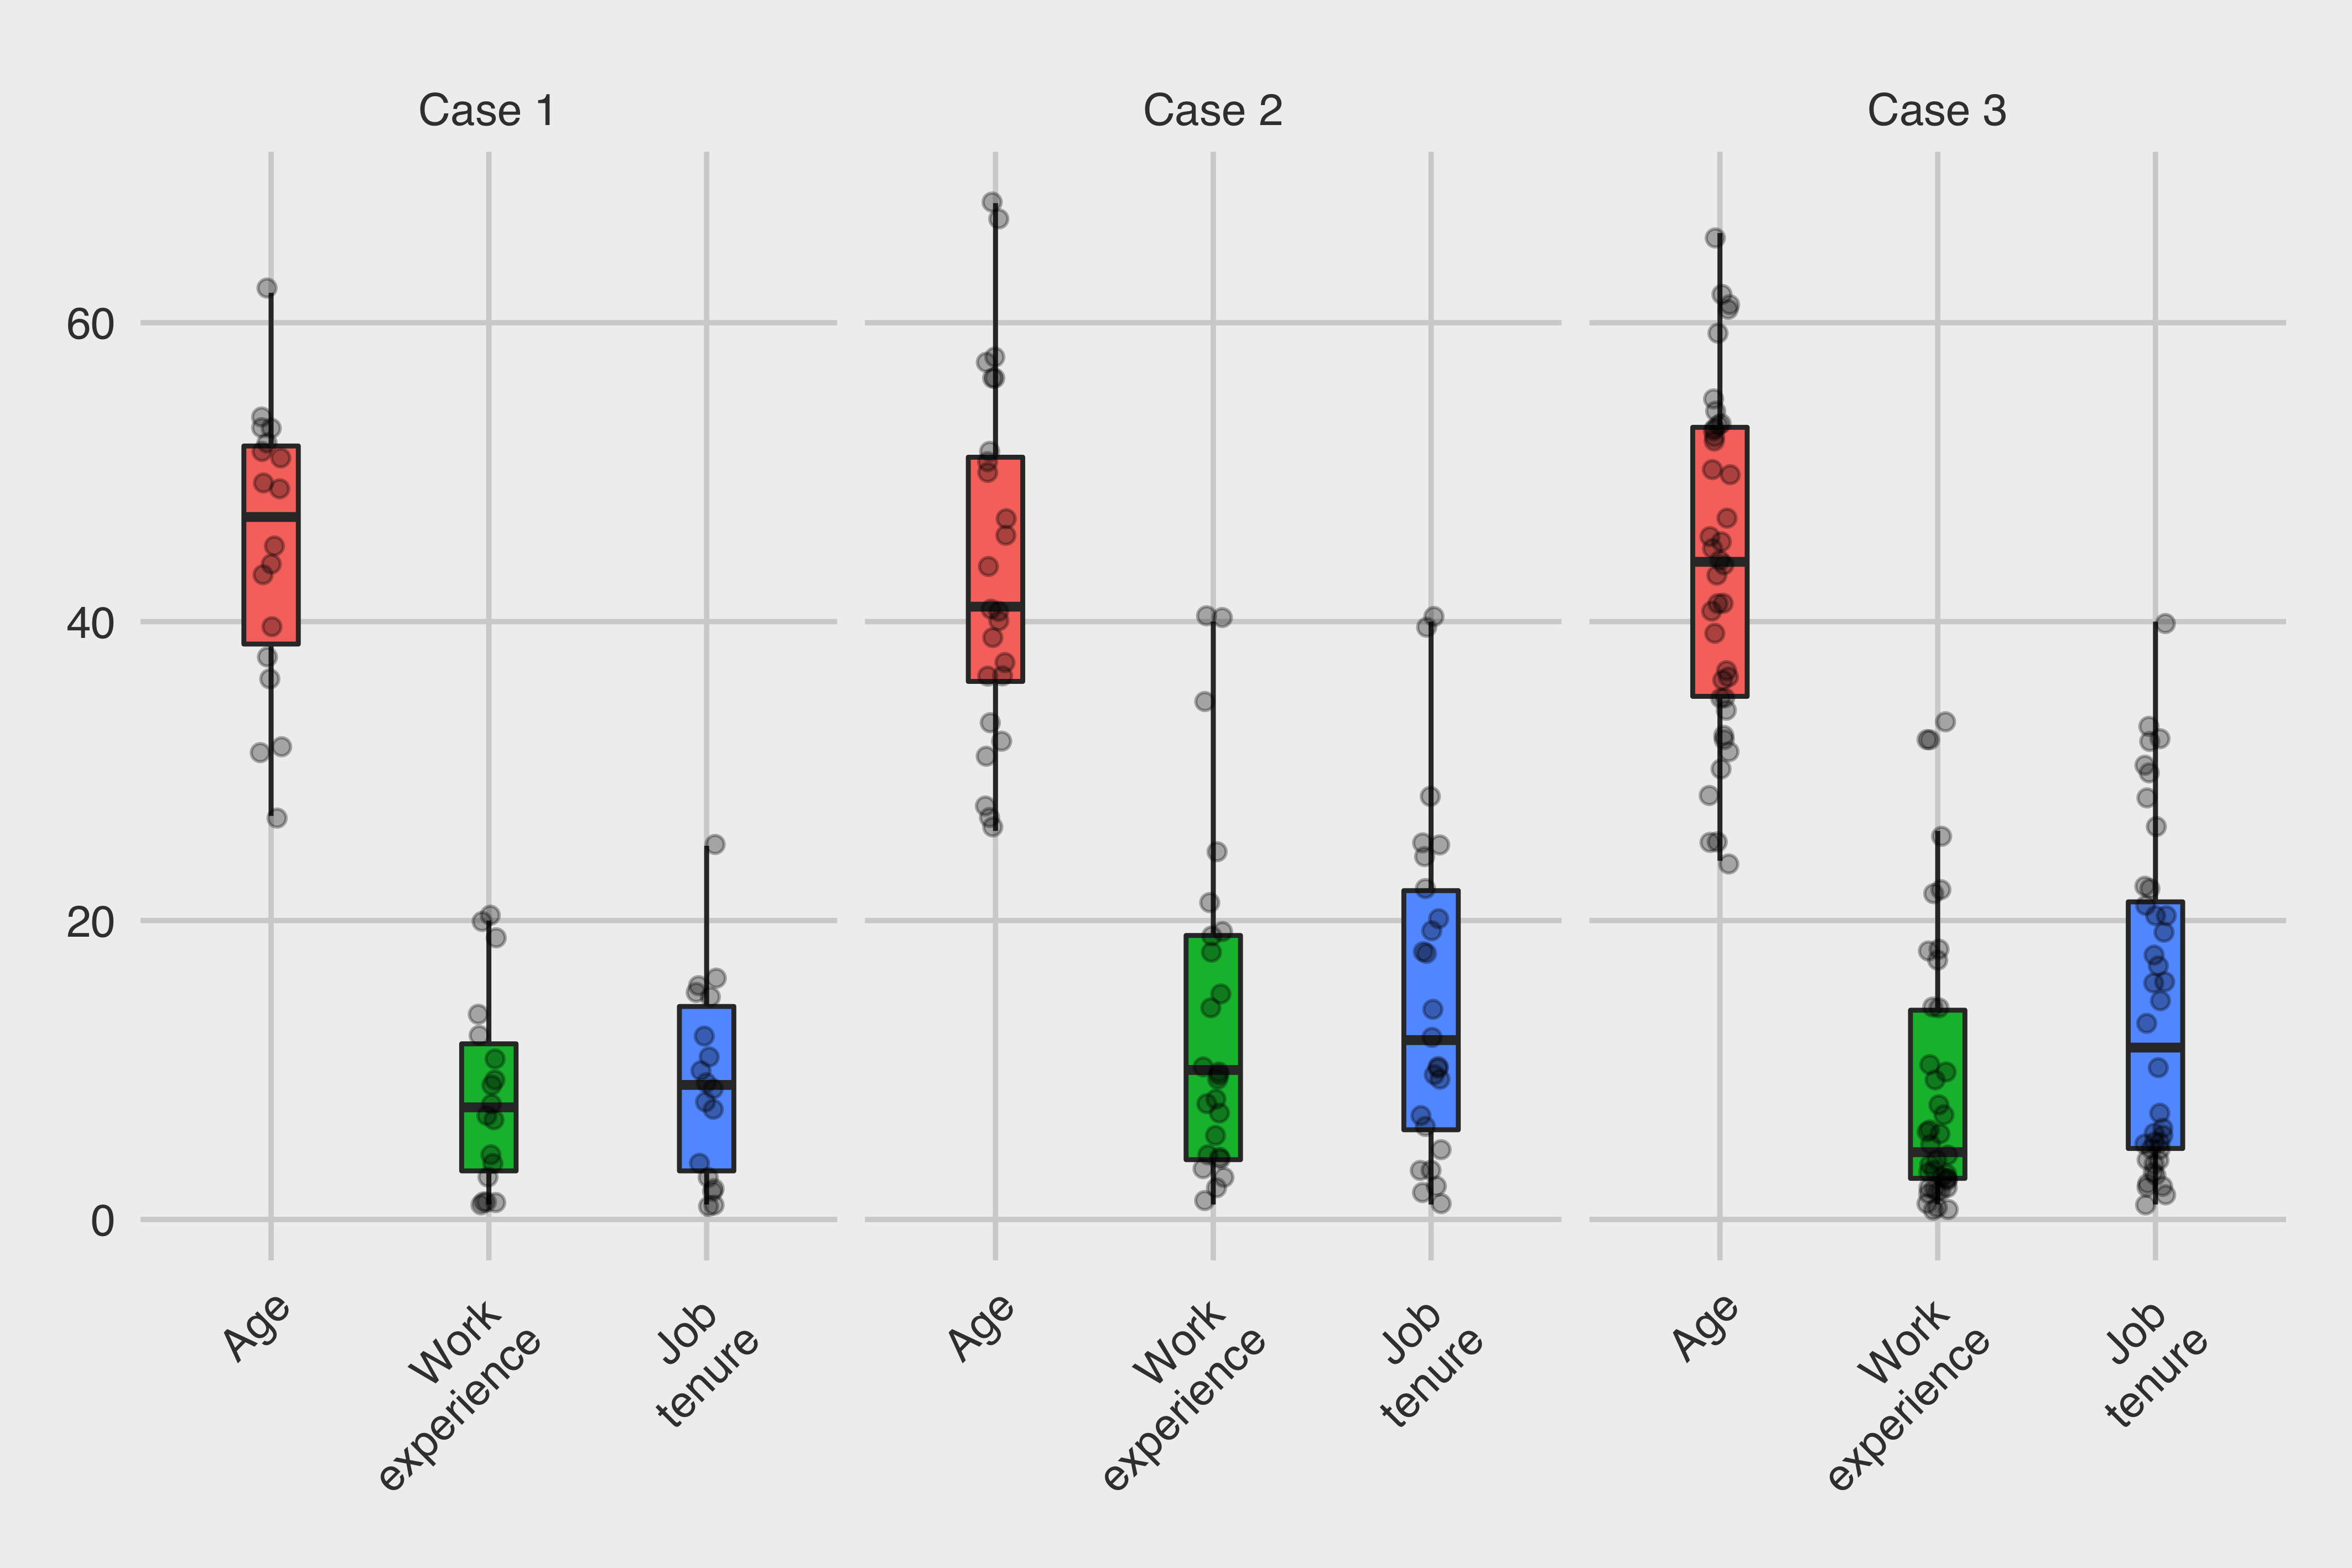
\includegraphics[width=1\linewidth]{Images/age_demographics.png}
\caption{Age, work experience, and tenure.}
%\label{fig:age} 
\end{subfigure}

\begin{subfigure}[b]{0.7\textwidth}
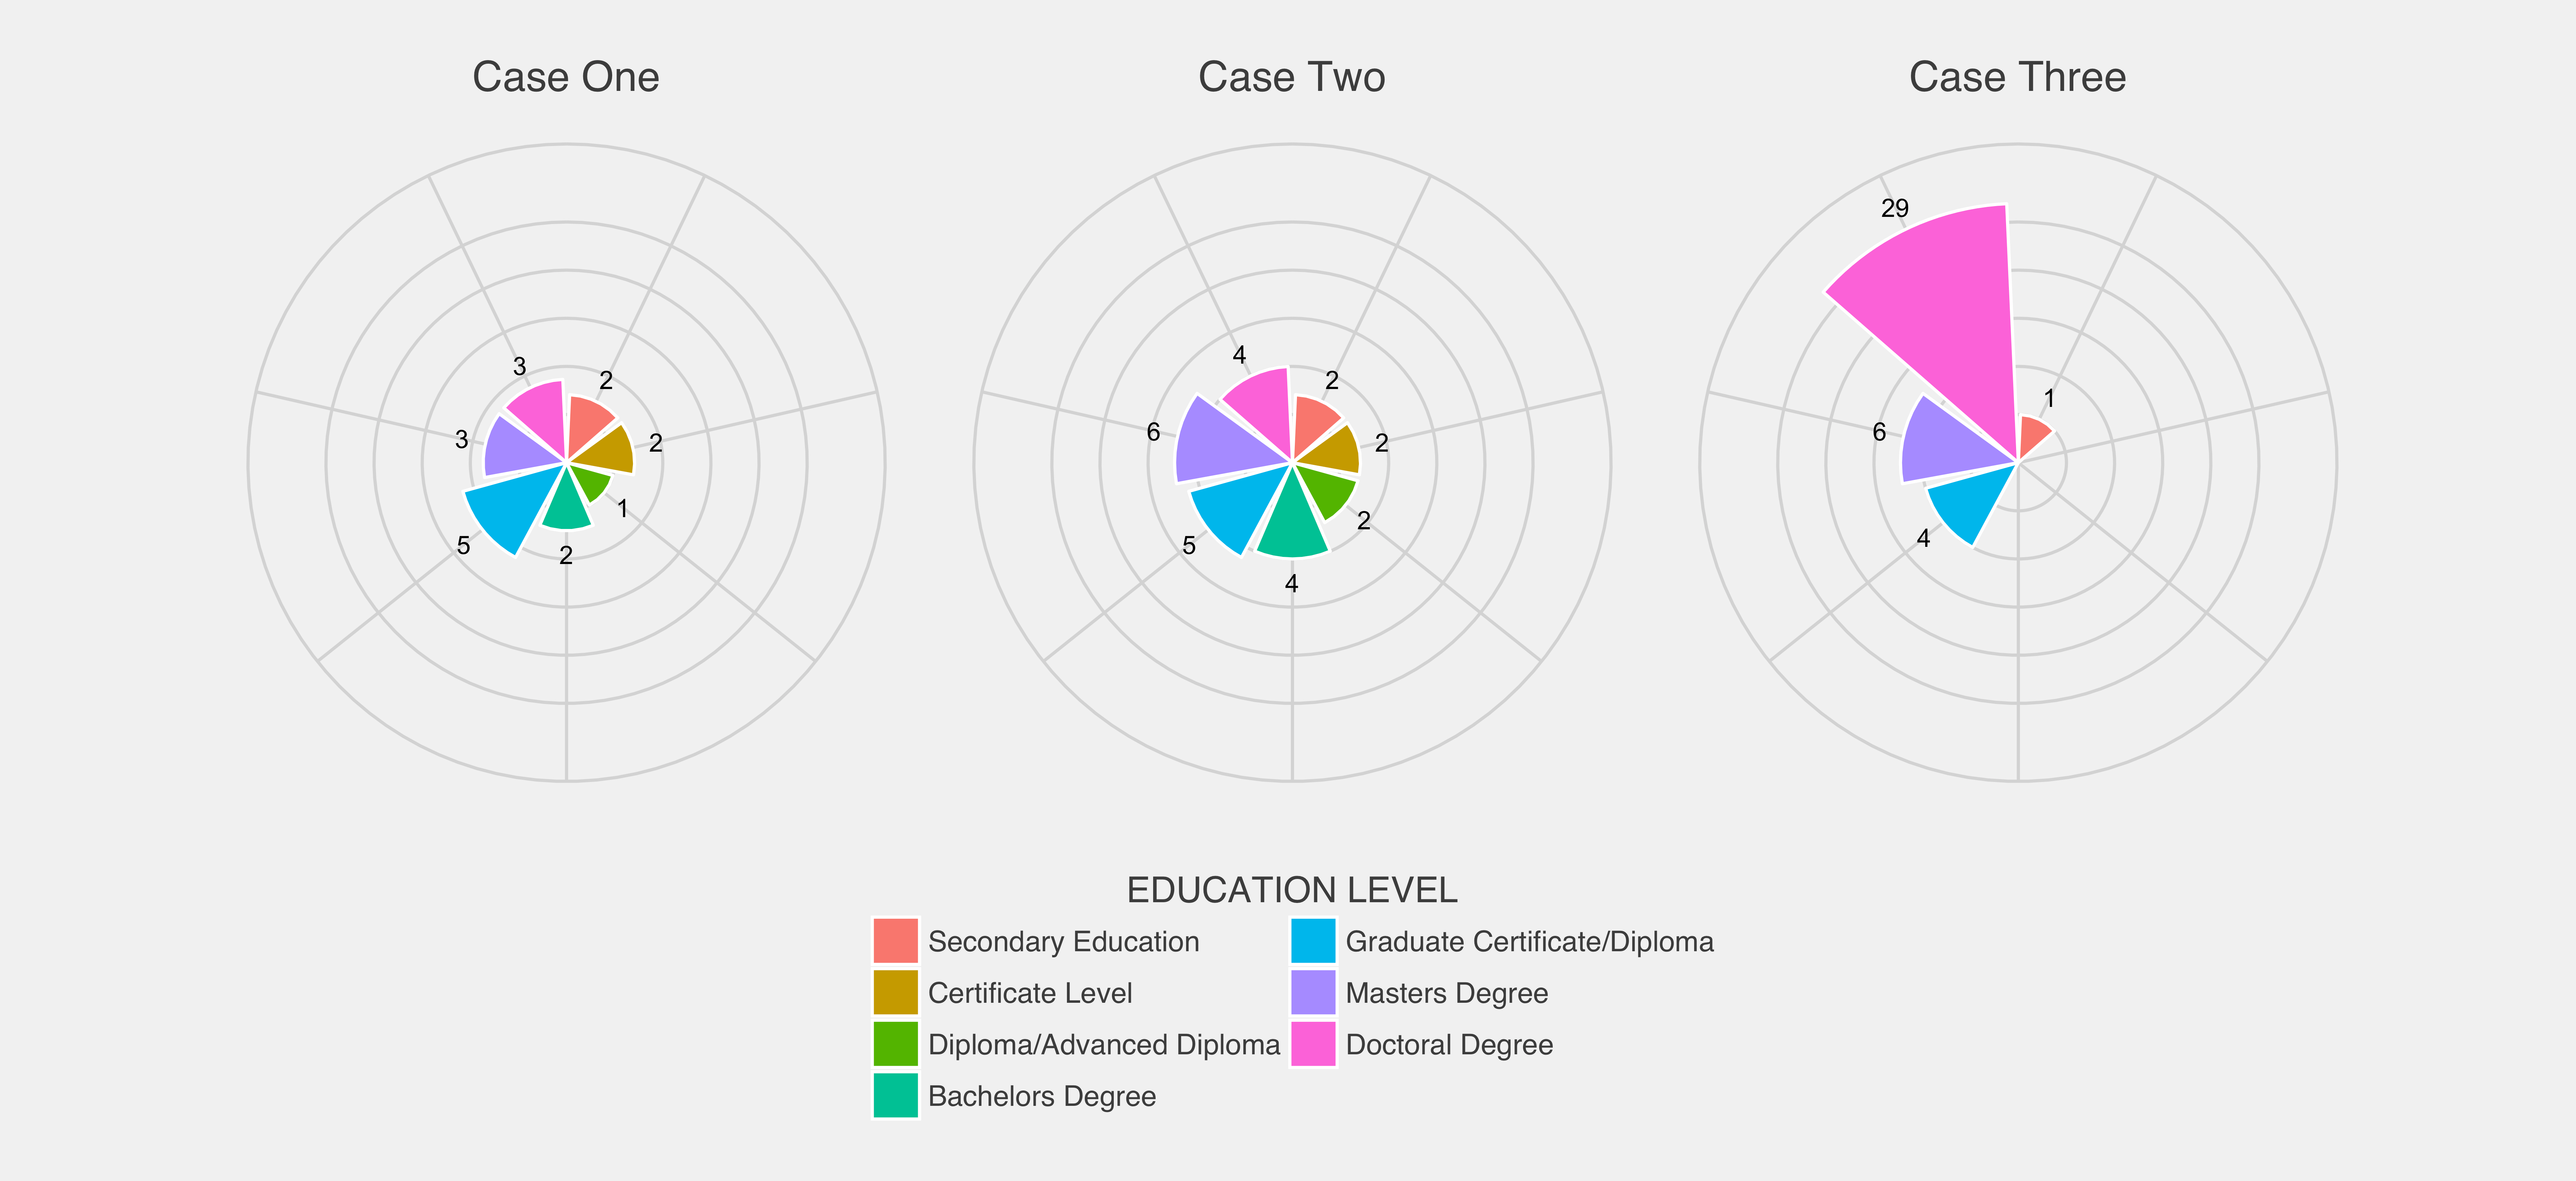
\includegraphics[width=1\linewidth]{Images/ed_level.png}
\caption{Education level}
%\label{fig:ed_level}
\end{subfigure}

\begin{subfigure}[b]{0.7\textwidth}
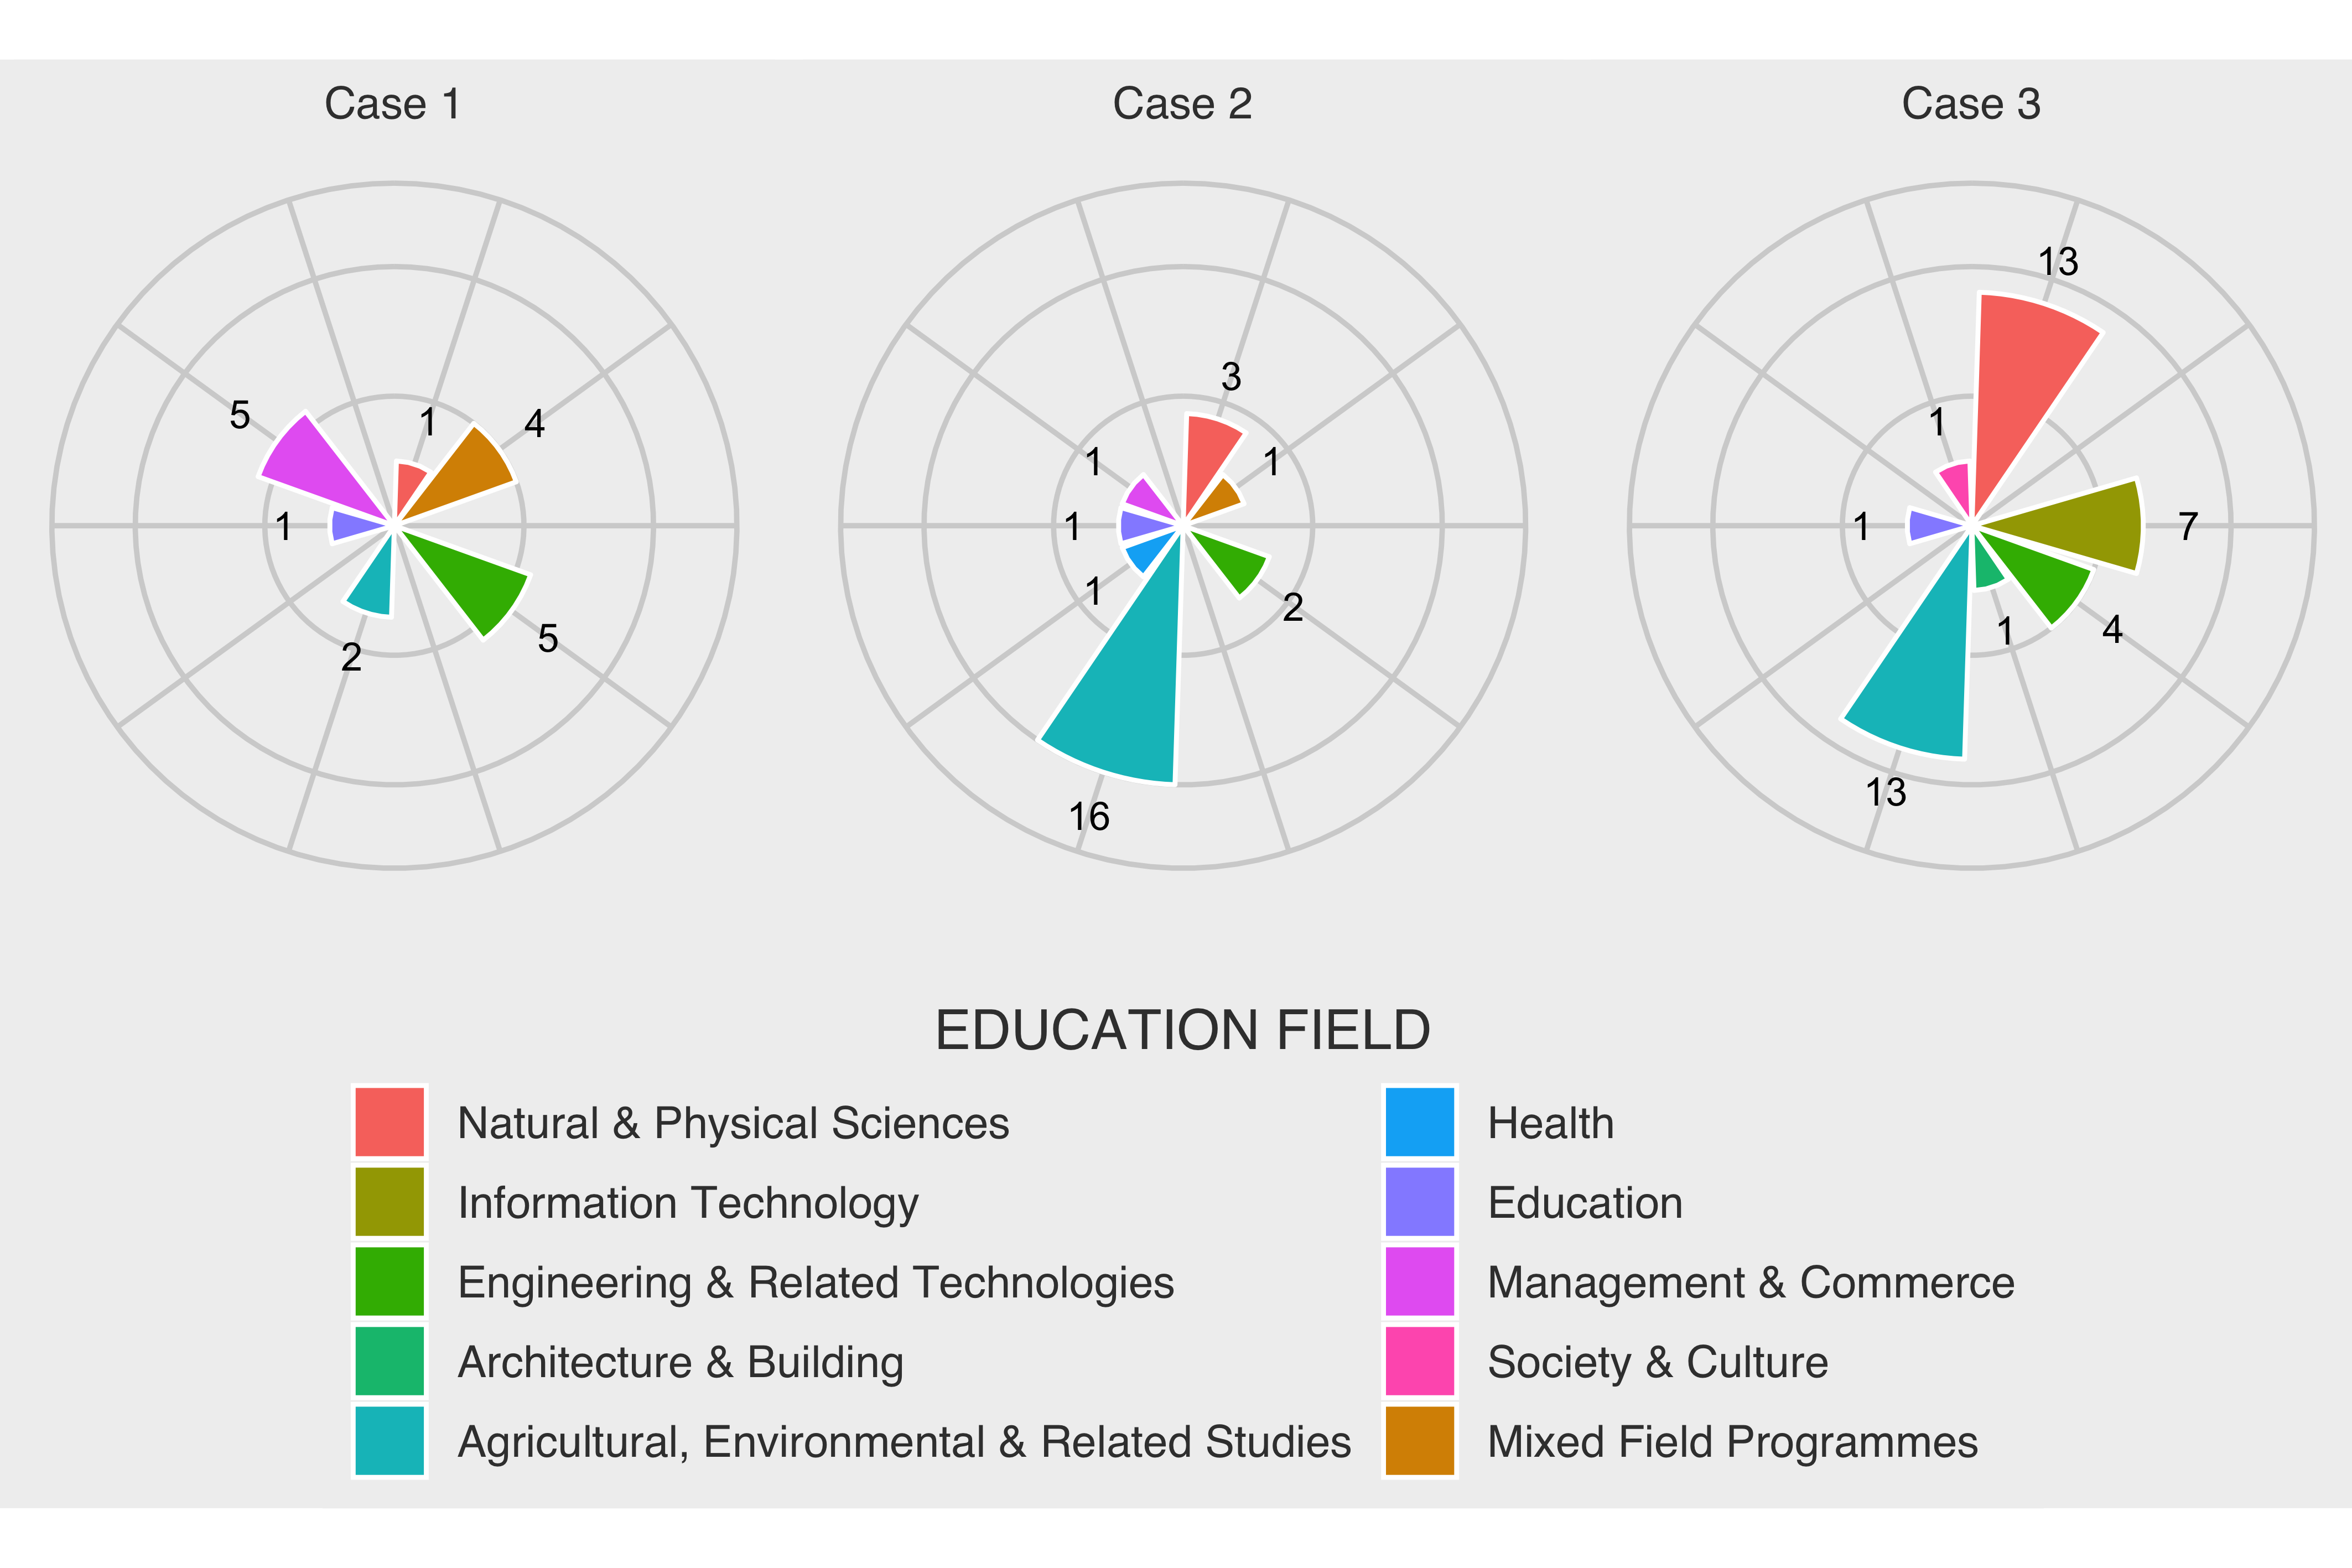
\includegraphics[width=1\linewidth]{Images/ed_field.png}
\caption{Education field.}
%\label{fig:ed_field}
\end{subfigure}

\caption[Demographic information for each case]{Demographic information for the three open innovation cases.}
\label{fig:demographics}
\end{figure}


\subsection{Psychological attributes}

Figure \ref{fig:psycho} shows the range of different psychological attributes in each case (three of the \enquote{Big Five} personality traits, work motivation, job-related and creative self-efficacy, and identification with workgroup/employer/open innovation partnership). 


\begin{landscape}
\begin{figure*}
\centering
\begin{subfigure}[b]{0.7\textwidth}
\centering
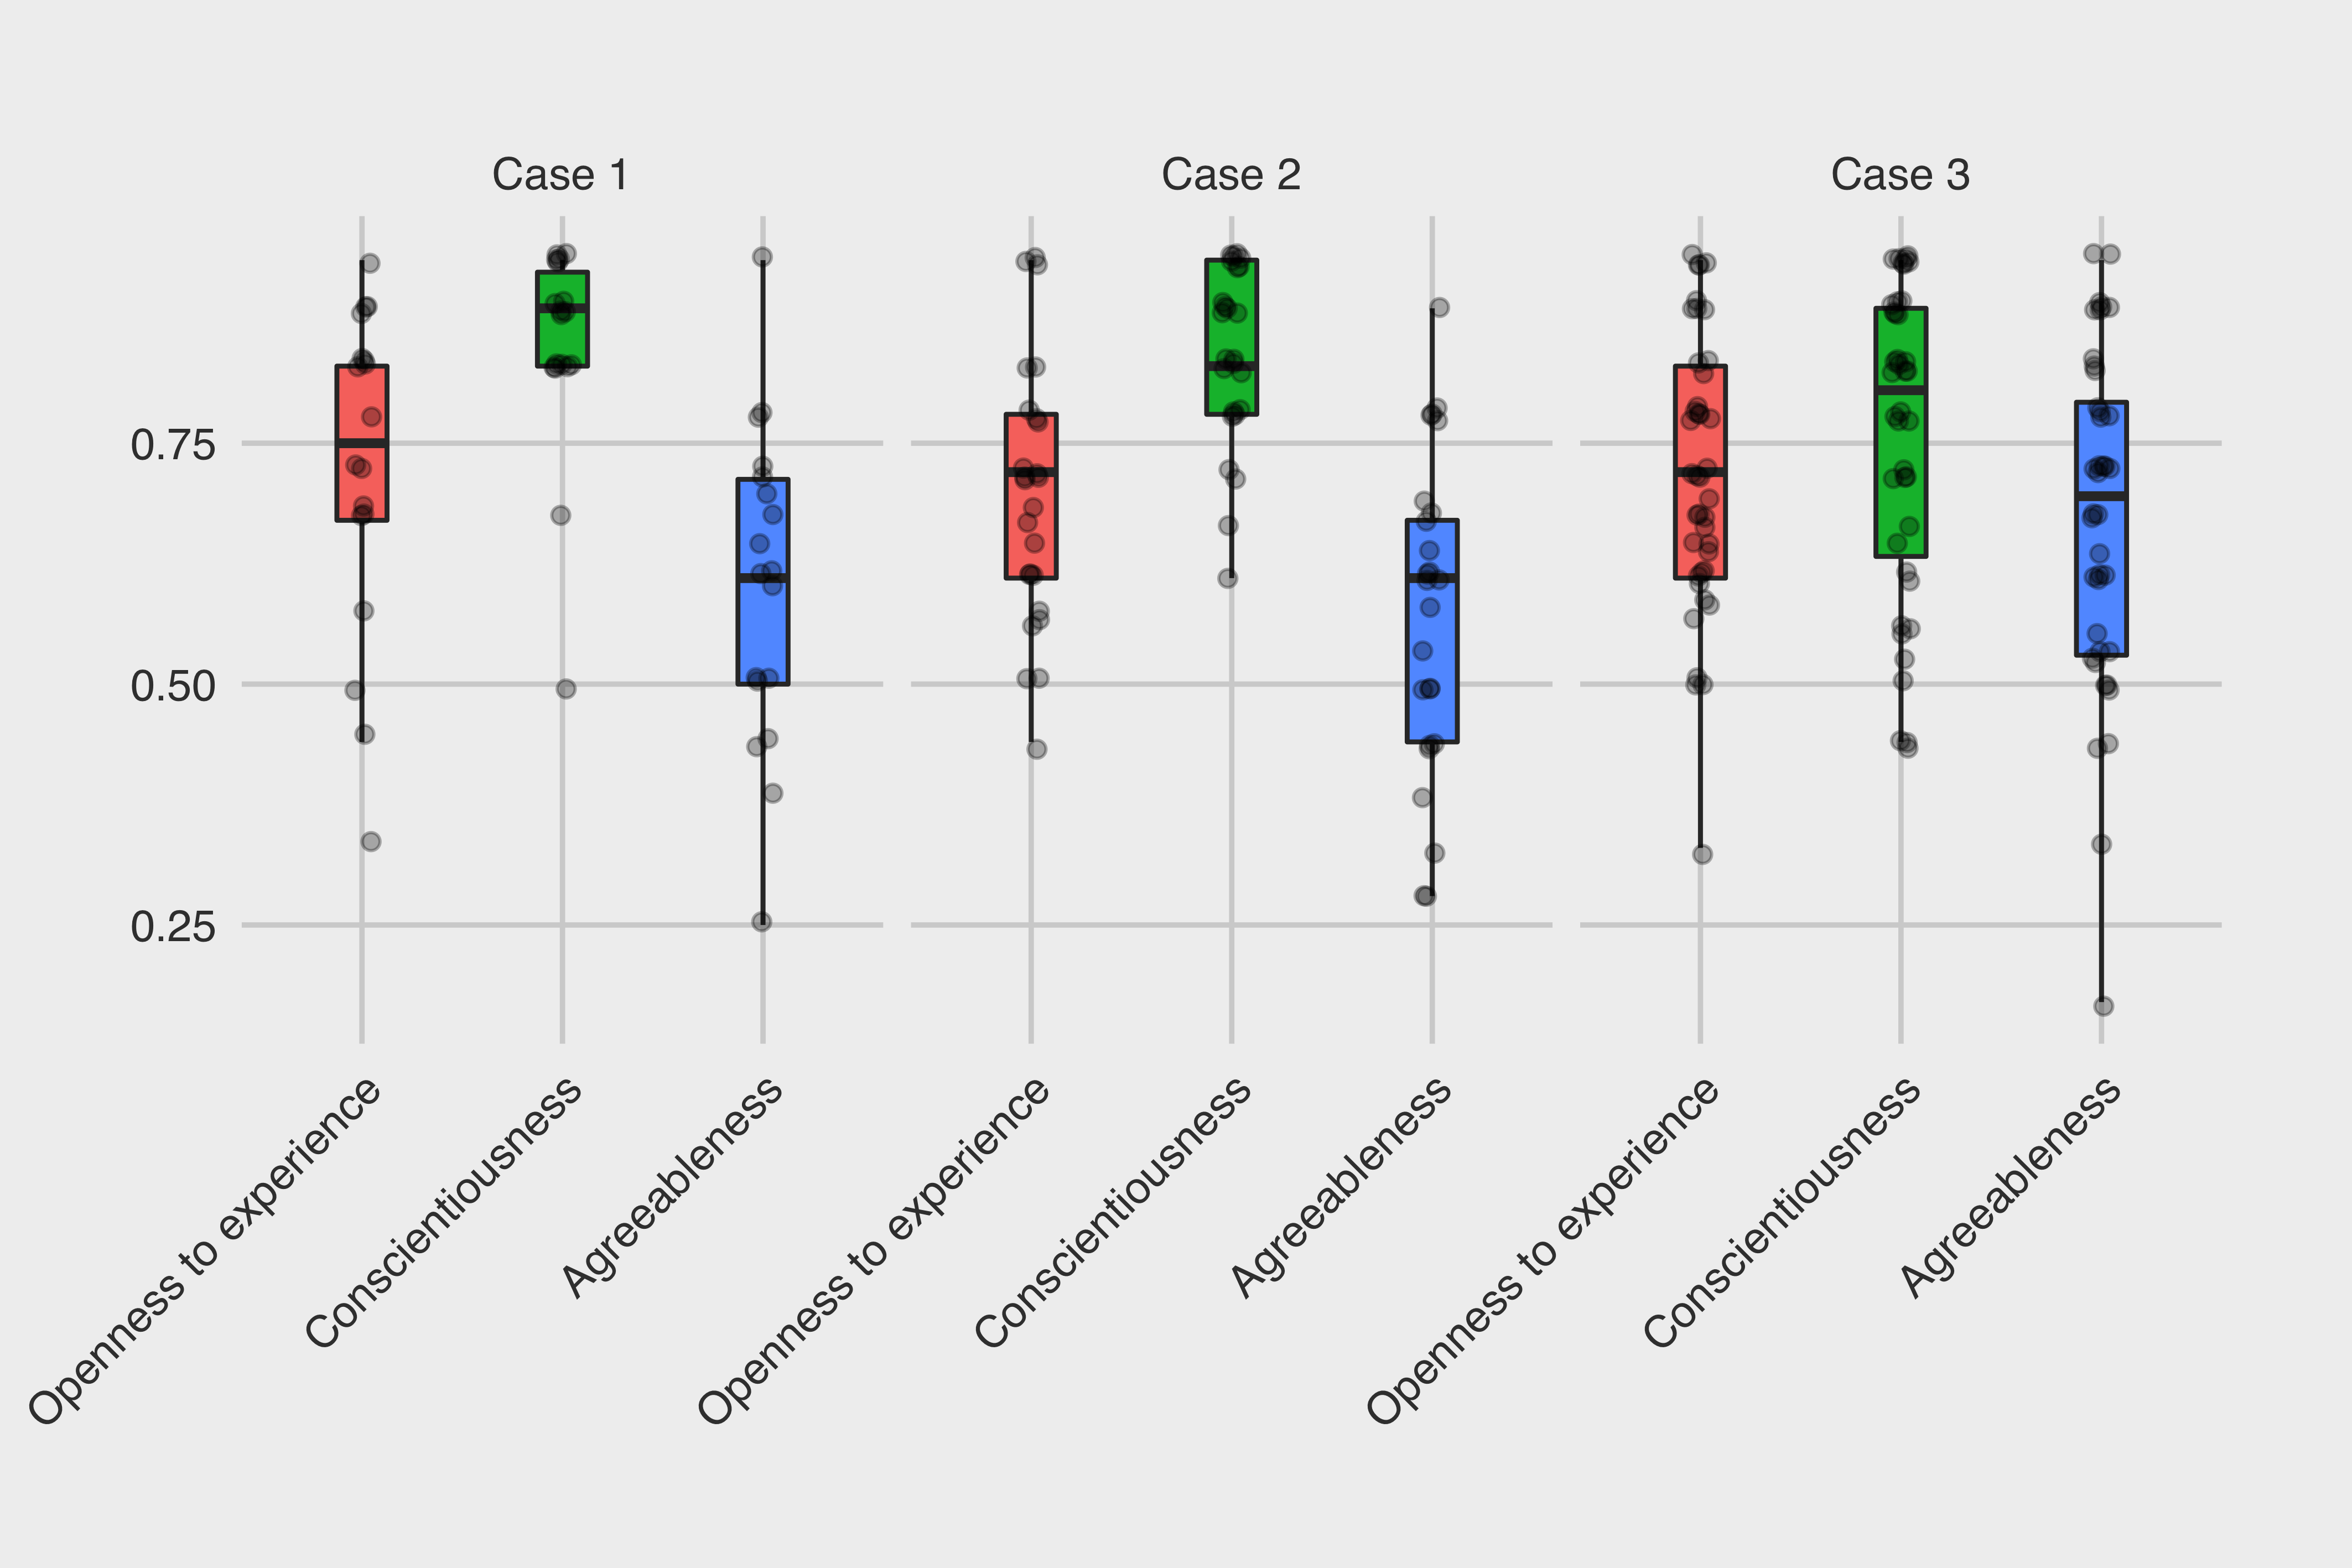
\includegraphics[width=\textwidth]{Images/personality_case.png}
\caption[]%
{{\small Personality traits.}}    
\label{fig:personality}
\end{subfigure}
\hfill
\begin{subfigure}[b]{0.7\textwidth}  
\centering 
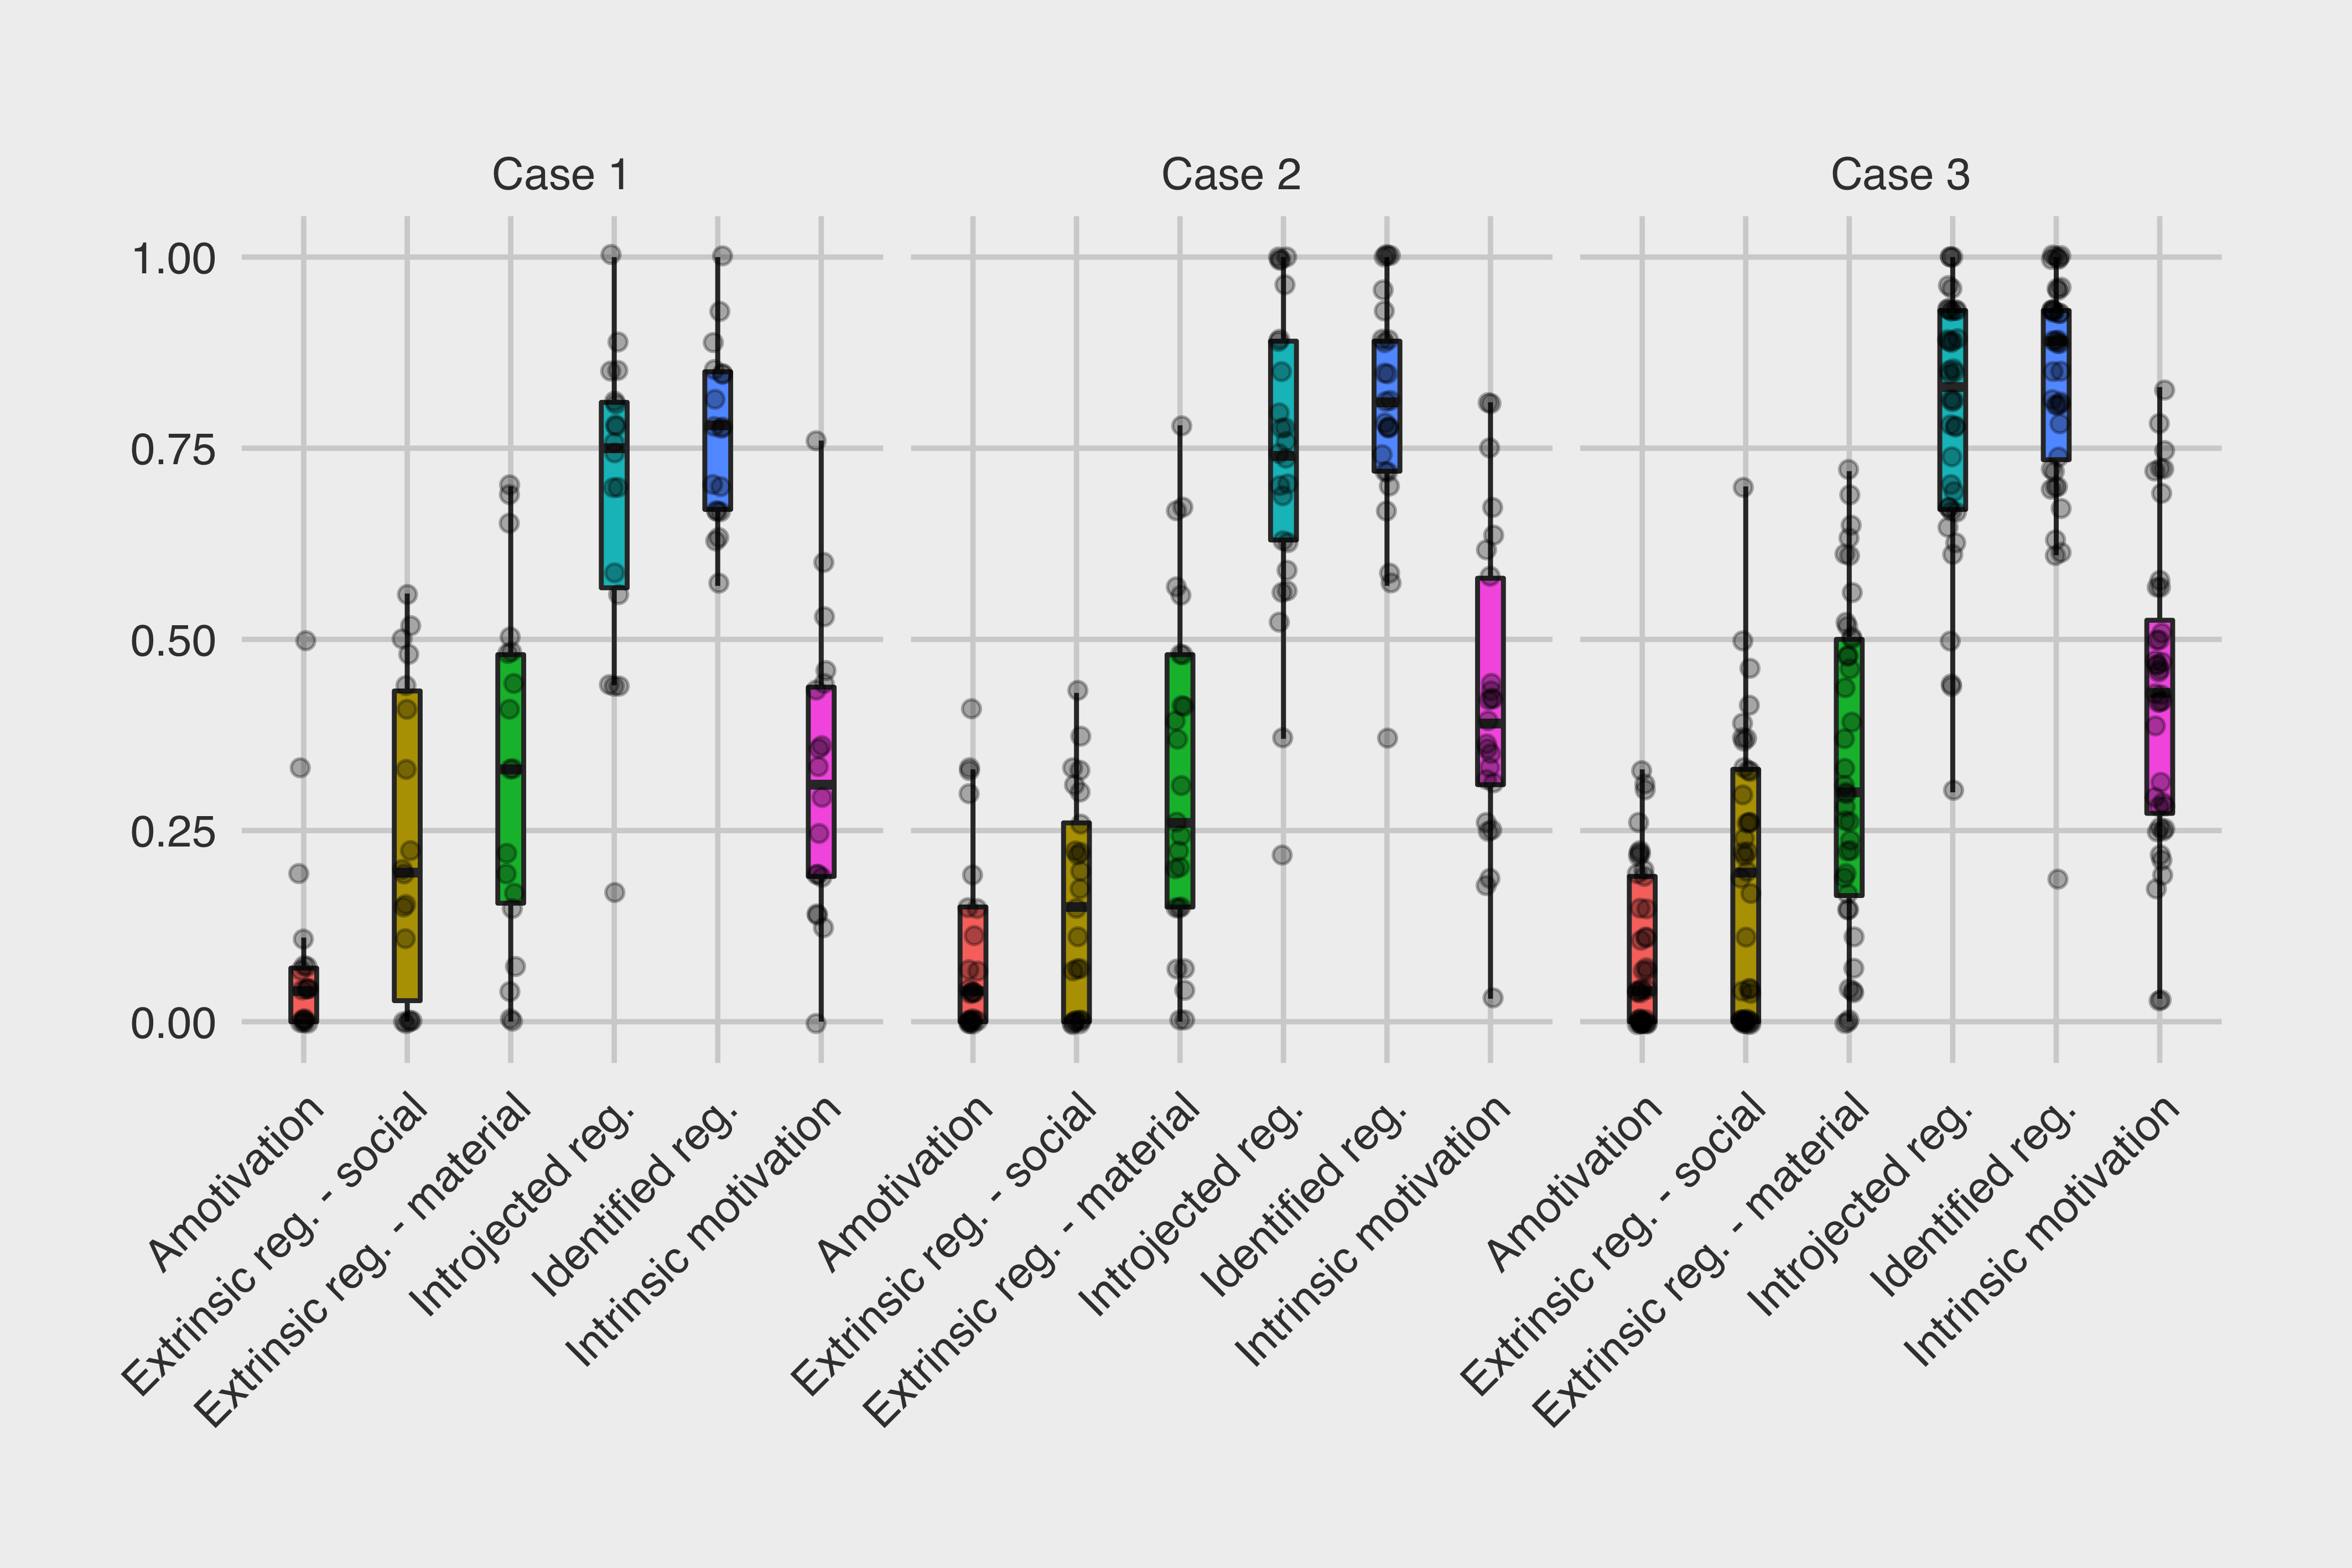
\includegraphics[width=\textwidth]{Images/work_motivation_case.png}
\caption[]%
{{\small Work motivation.}}    
\label{fig:motivation}
\end{subfigure}
\vskip\baselineskip
\begin{subfigure}[b]{0.7\textwidth}   
\centering 
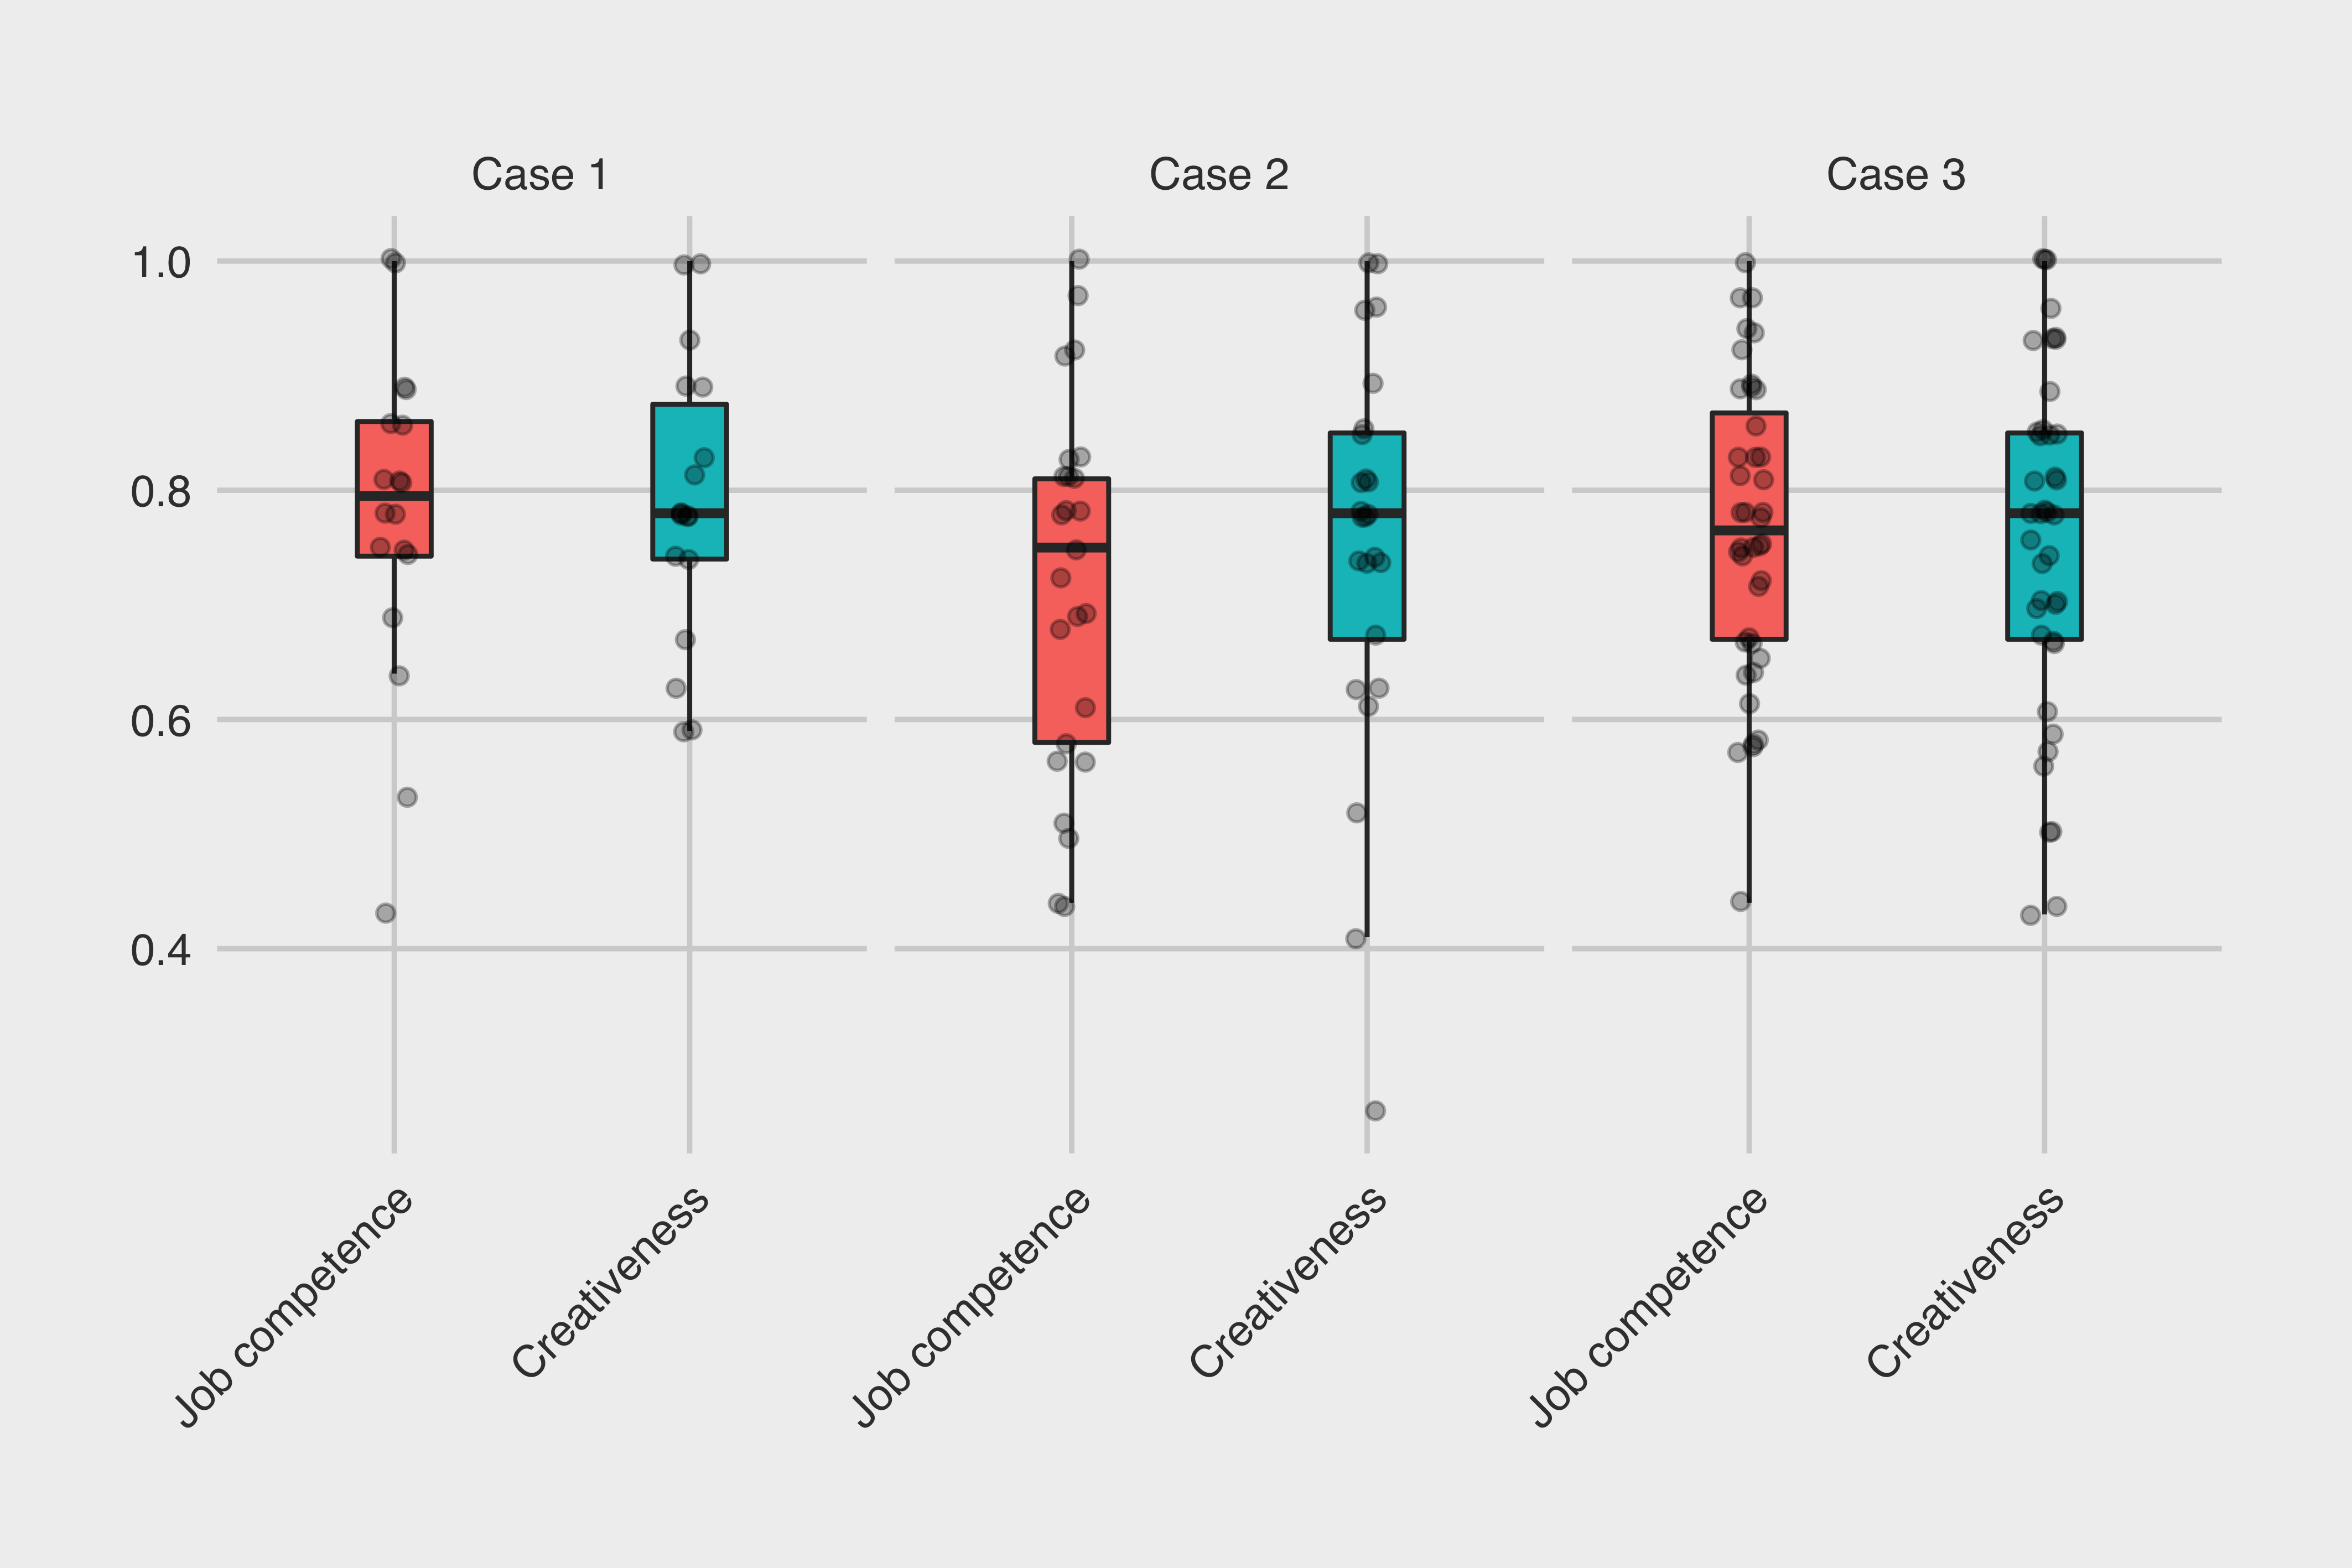
\includegraphics[width=\textwidth]{Images/efficacy_case.png}
\caption[]%
{{\small Self-efficacy.}}    
\label{fig:efficacy}
\end{subfigure}
\hfill
\begin{subfigure}[b]{0.7\textwidth}   
\centering 
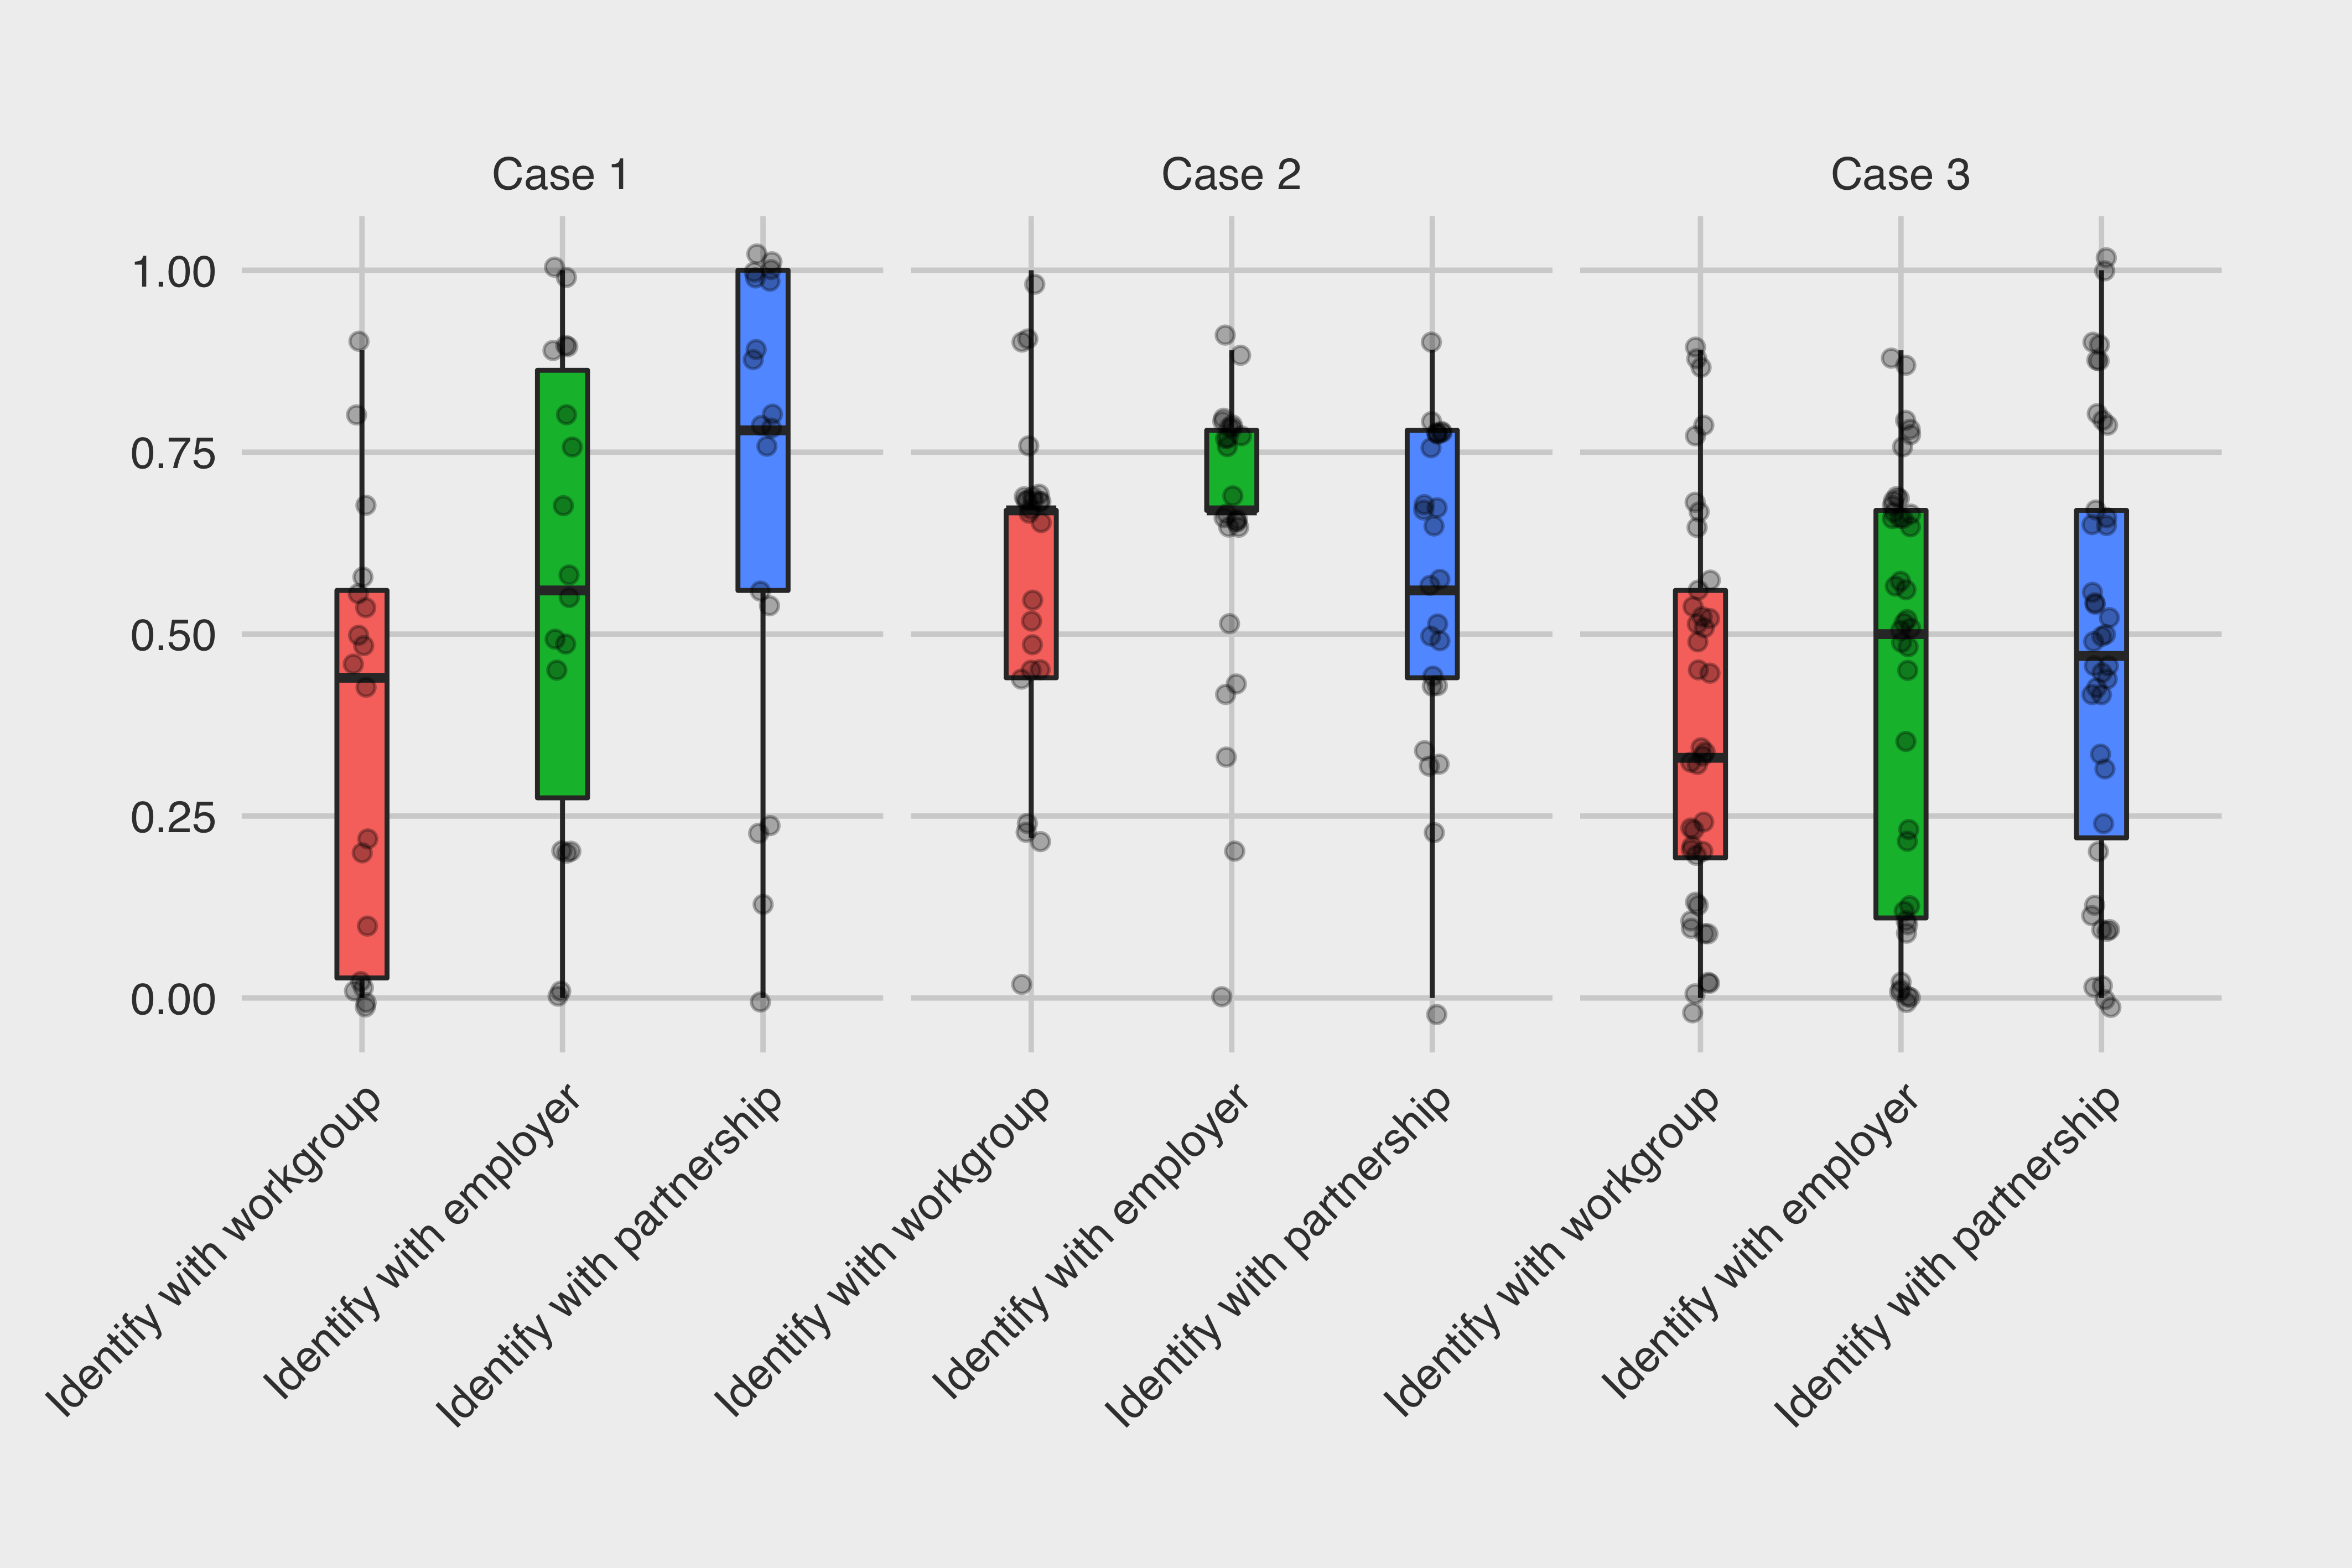
\includegraphics[width=\textwidth]{Images/identification_case.png}
\caption[]%
{{\small Social identity.}}    
\label{fig:identification}
\end{subfigure}
\caption[Psychological attributes of case participants]
{\small {Psychological attributes of case participants.}} 
\label{fig:psycho}
\end{figure*}
\end{landscape}

\subsection{Geographic proximity}

The geographic spread of participants has implications for tacit knowledge sharing, which generally happens through face-to-face interactions. Participants who are not nearby have fewer opportunities to exchange tacit knowledge with one another. All three cases involve participants based in other countries. Figure \ref{fig:spherical} depicts matrices that show the spherical distance between participants in each case (based on reported workplace postcodes). Case 1 has participants local to each other, in another part of Australia, and one based on another continent. Participants in Case 2 are more spread out. While some participants are local, others are located much further afield, either in another part of the country or another country or continent altogether. Participants in Case 3 are also spread out, with some located on separate continents.  \medskip

\begin{figure}[h!]
\centering
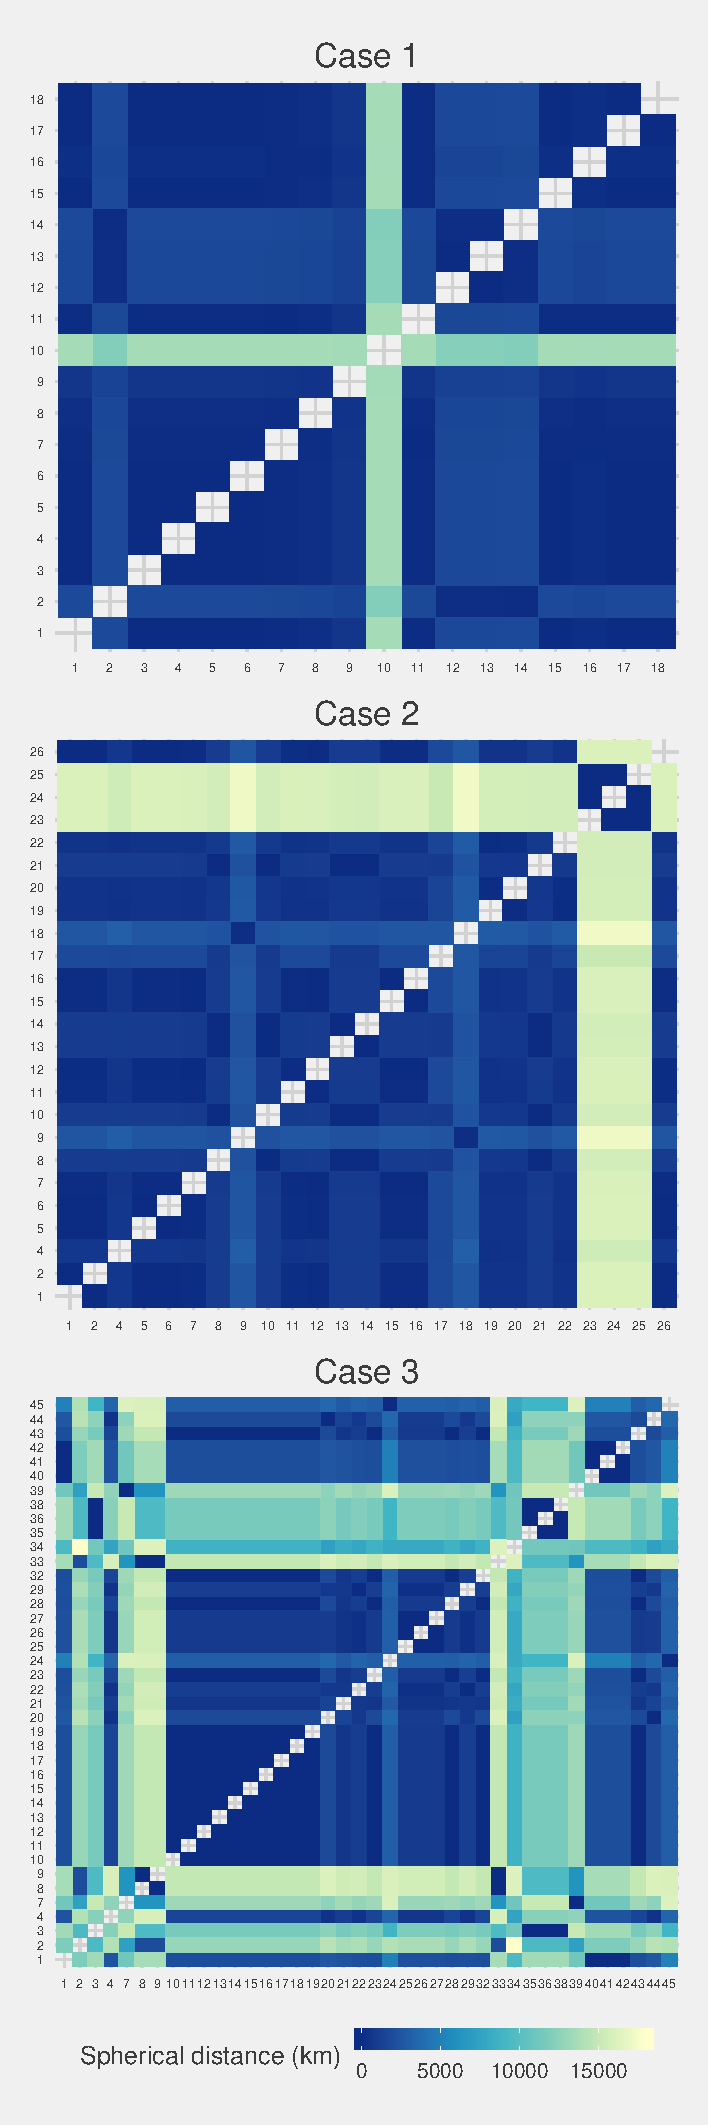
\includegraphics[width = 0.5\linewidth]{Images/proximity.pdf}
\caption[Geographical separation between participants]{Geographical separation between participants.}
\label{fig:spherical}
\end{figure}

\subsection{Network diagrams}

Figures \ref{fig:network_case_1} to \ref{fig:network_case_3} depict the tacit and explicit knowledge provision ties between participants within each case. Nodes are coloured by partner affiliation and sized according to their Everett-Valente brokerage score, where larger nodes have greater access to diverse knowledge. The direction of knowledge flow is indicated by edge shading (flows from light to dark). Edge colours reflect the geographical separation between nodes (lighter colours indicate greater separation). \medskip

Each case has a few highly central actors, some of whom are particularly dominant. The graph densities indicate that the bulk of the knowledge provided in Case 1 is explicit. There is more of an even balance in Case 2, where tacit knowledge provision edges out explicit knowledge provision. Though Case 3 is also more balanced, the density of the explicit knowledge network is slightly higher than that for the tacit knowledge provision network. The graph densities appear to reflect the maturity of each open innovation partnership - the more mature cases tend to have higher graph densities. Edge colours indicate the distance between connected nodes. Lighter colours mean greater separation between nodes. What is notable is the geographic separation between nodes exchanging tacit knowledge. It indicates some participants make a considerable effort to meet face-to-face despite working far apart. \medskip

\begin{sidewaysfigure}
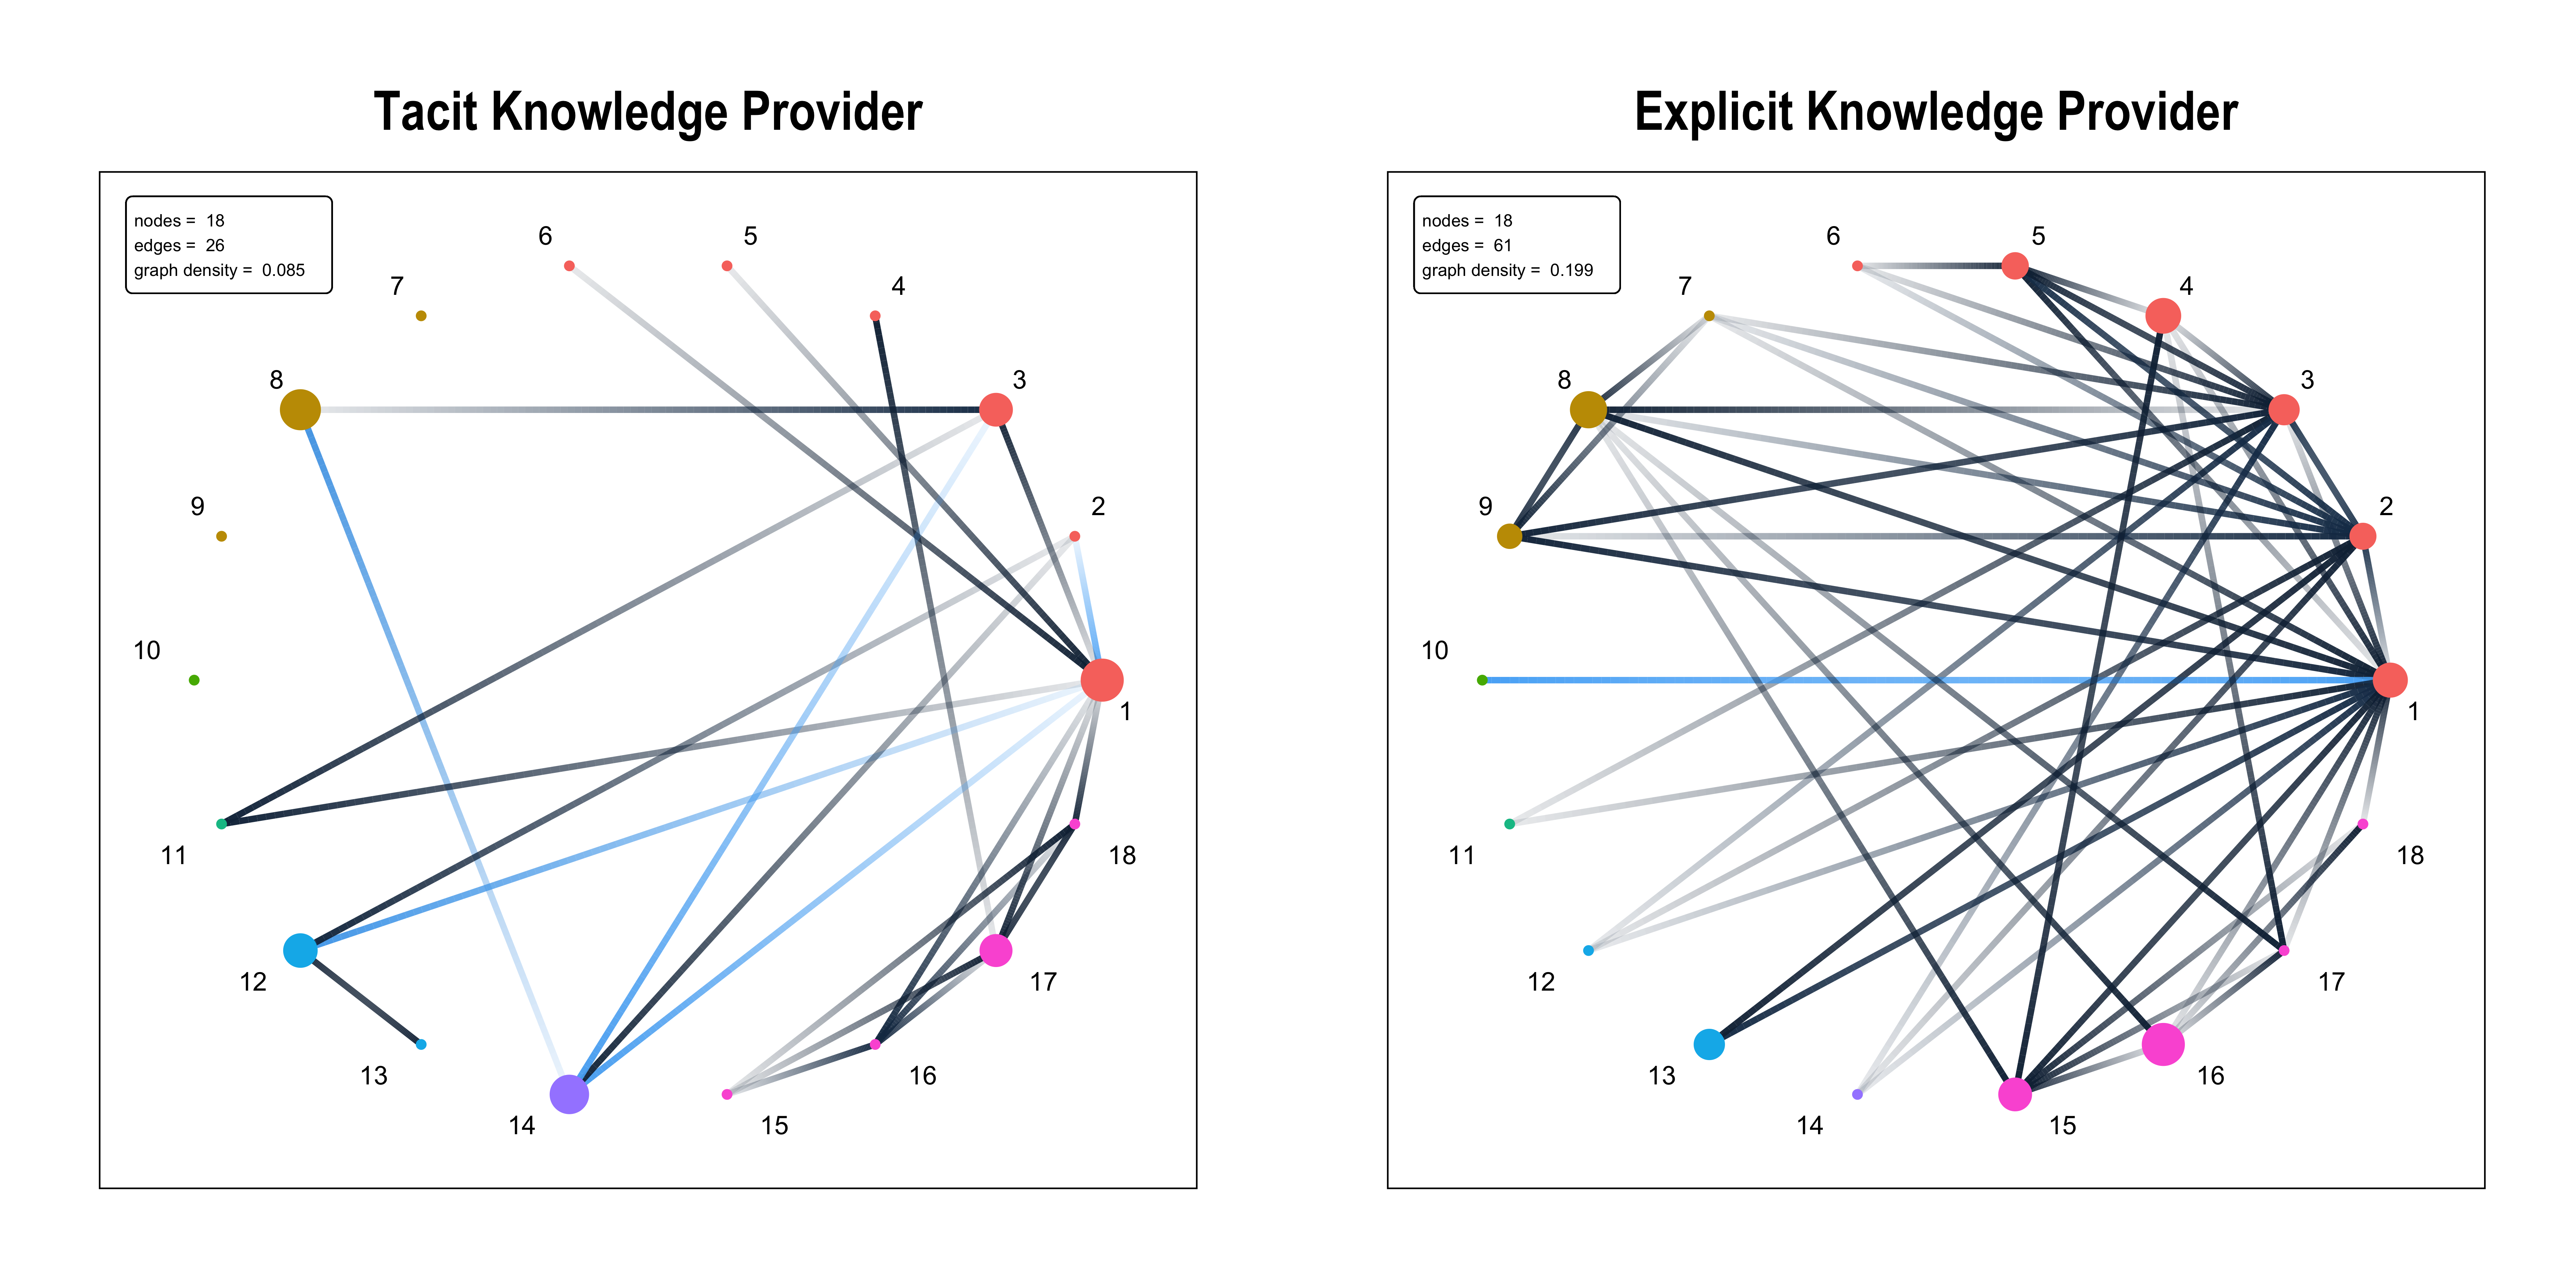
\includegraphics[width=1\linewidth]{Images/networks_case_1.png}
\caption[Knowledge networks for Case 1]{Knowledge networks for Case 1 (see text for an explanation of the different graphical representations).}
\label{fig:network_case_1} 
\end{sidewaysfigure}

\begin{sidewaysfigure}
\includegraphics[width=1\linewidth]{Images/networks_case_2.png}
\caption[Knowledge networks for Case 2]{Knowledge networks for Case 2 (see text for an explanation of the different graphical representations).}
\label{fig:network_case_2} 
\end{sidewaysfigure}

\begin{sidewaysfigure}
\includegraphics[width=1\linewidth]{Images/networks_case_3.png}
\caption[Knowledge networks for Case 3]{Knowledge networks for Case 3 (see text for an explanation of the different graphical representations).}. 
\label{fig:network_case_3} 
\end{sidewaysfigure}

\subsection{Broker roles}

Brokers are well placed to control the flow of knowledge across organisational boundaries. By examining broker roles, one can assess knowledge diffusion in open innovation partnerships. Figure \ref{fig:gf_brokerage} presents a breakdown of \citet{gould1989structures} broker roles by knowledge type in each case (refer to Table \ref{tab:ergm_params} for an explanation of these roles).  \medskip

The mix of broker roles reveals something about knowledge sharing behaviour in each case. Looking at Case 1, the liaison broker role is dominant in the explicit knowledge provider network, indicating participants are happy to pass on explicit knowledge to other partner organisations. Some participants operate in a representative broker role, suggesting they are open to sharing their organisation's explicit knowledge with third-parties. The representative broker role is dominant in the tacit knowledge provider network, indicating that participants are open to sharing their organisational know-how and expertise with third-parties. As to Case 2, the liaison role dominates both the explicit and tacit knowledge provider networks. Participants in Case 2 appear willing to pass on all types of knowledge to third-parties, a good sign of collaboration. The internal coordinator role dominates the explicit knowledge provider network in Case 3. Given that almost half the participants in Case 3 work for the same organisation, this is not surprising. The tacit knowledge provider network does not have a dominant broker role. Very few participants operate as itinerant brokers in any of the cases. \medskip

\begin{figure}
\centering
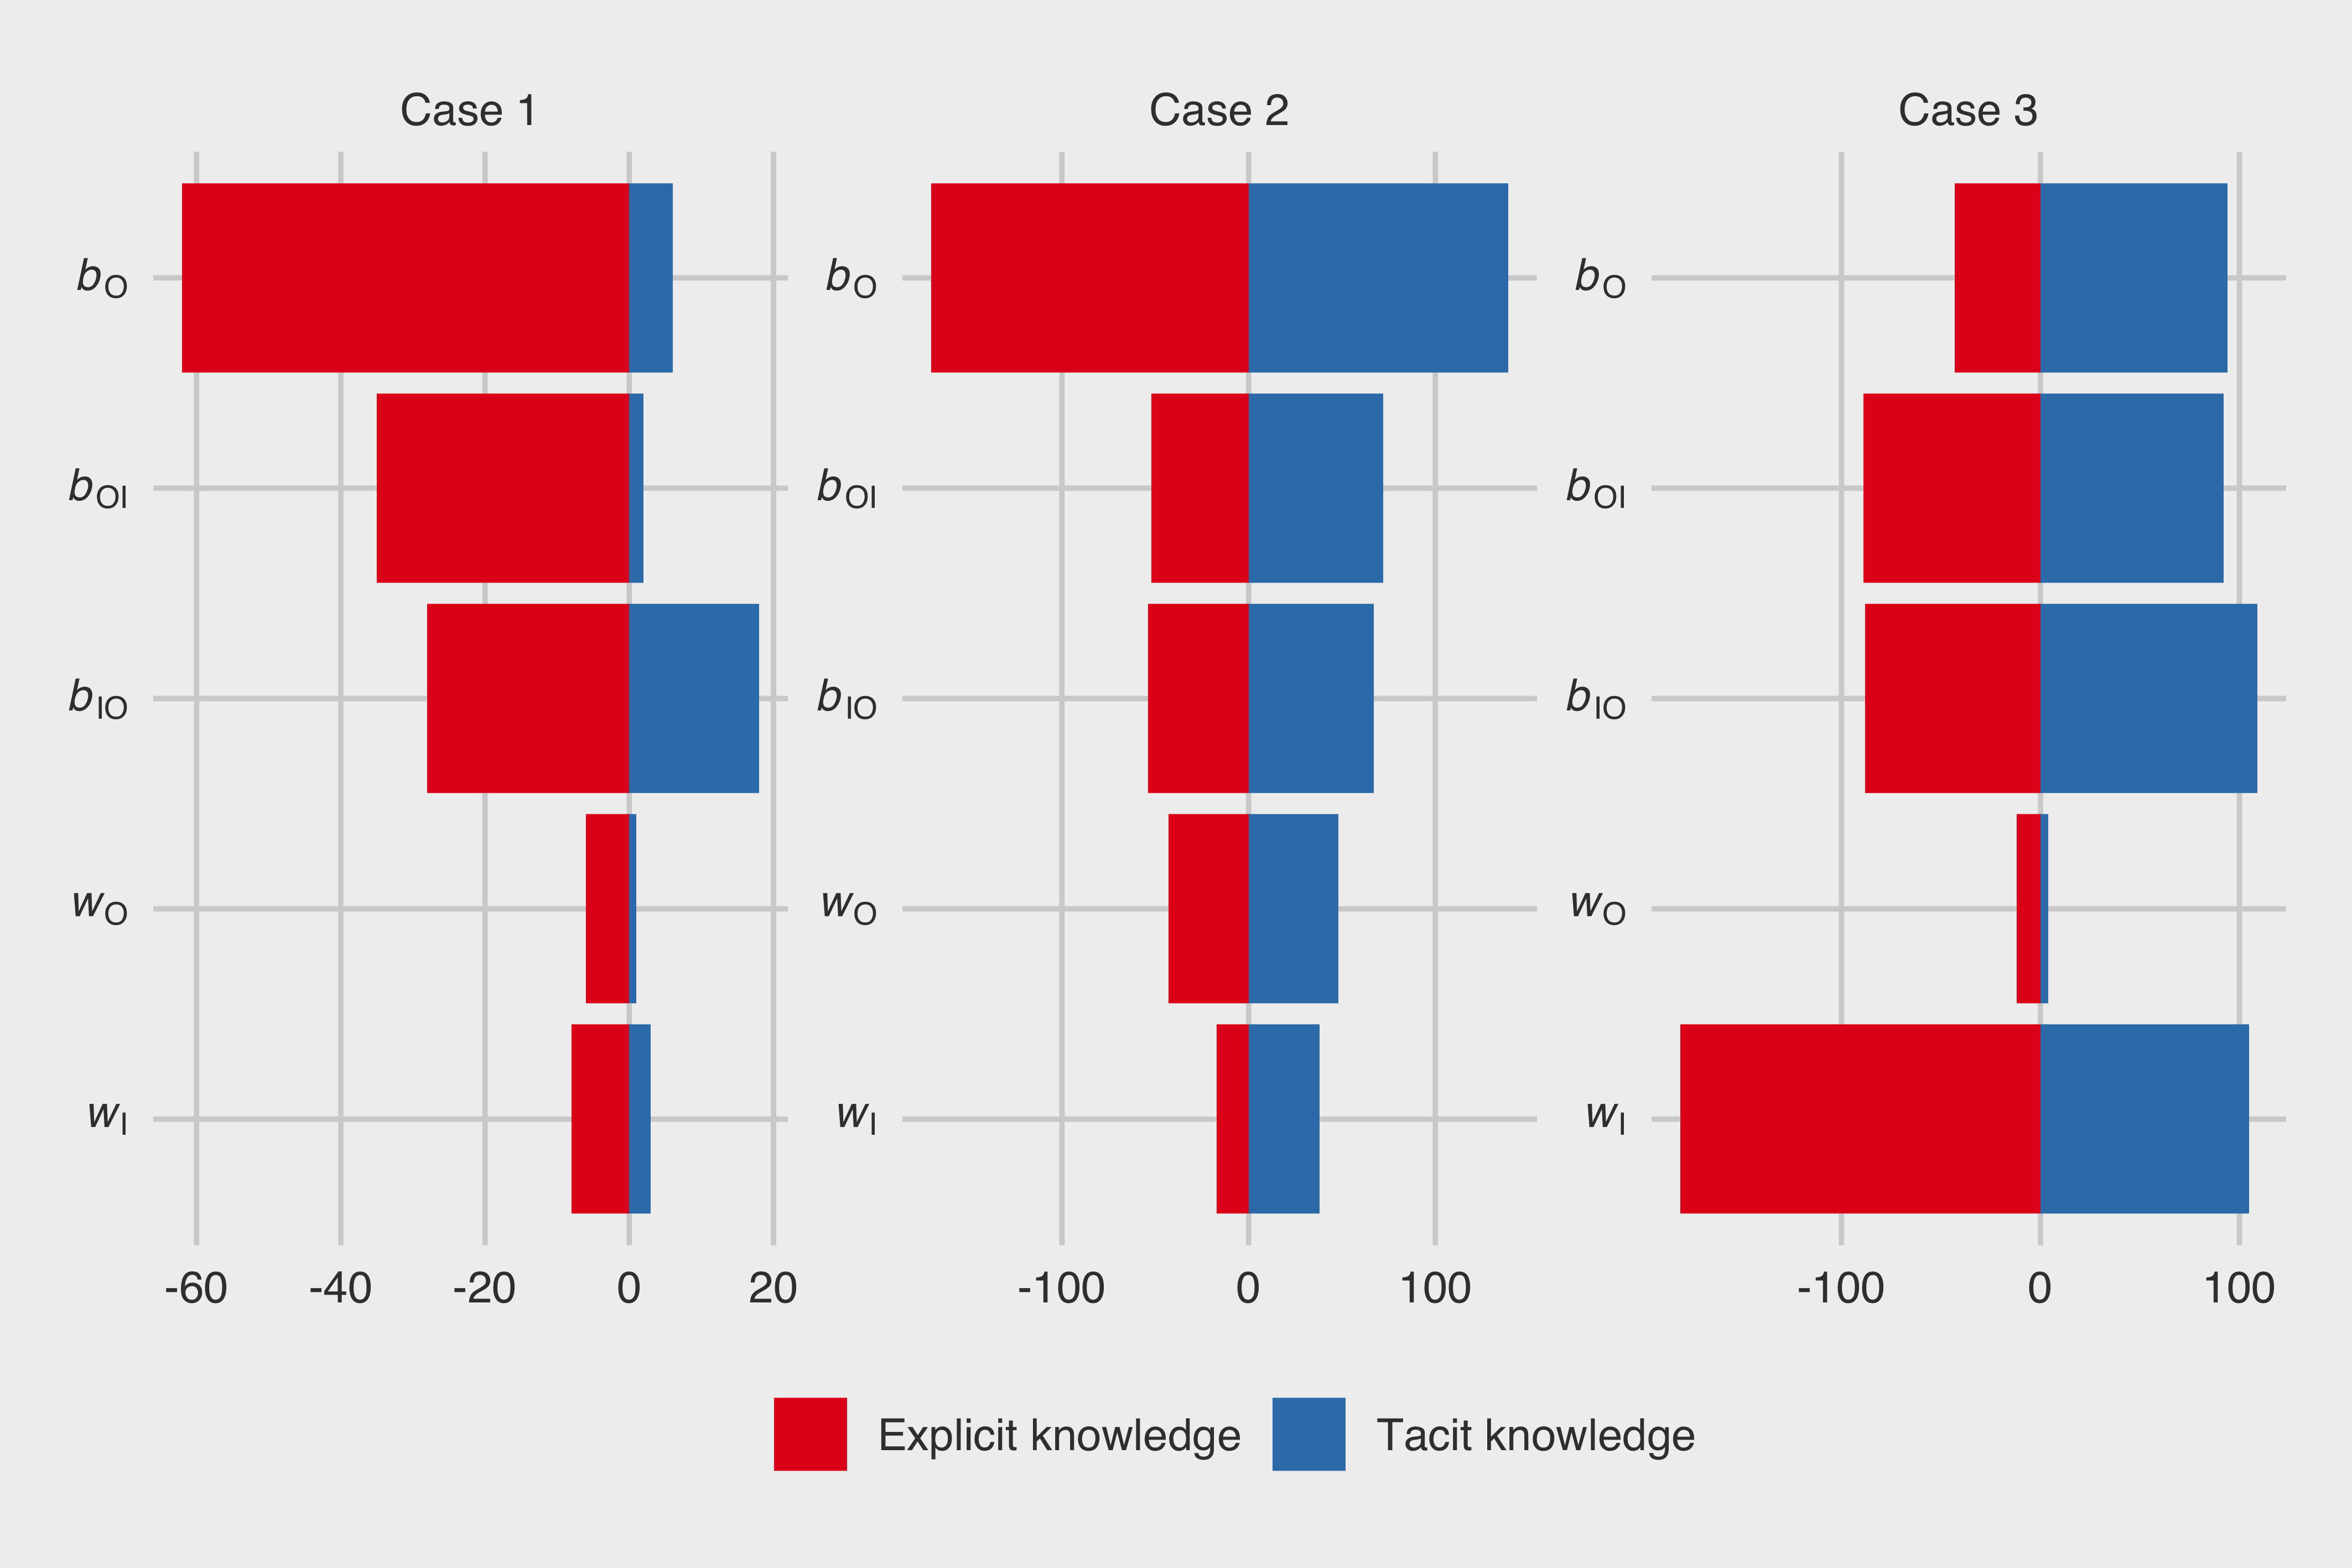
\includegraphics[width = \linewidth]{Images/gf_brokerage.png}
\caption[Breakdown of broker roles]{Breakdown of \citet{gould1989structures} broker roles. Note $w_I$ = internal coordinator role, $b_O$ = liaison role, $b_{OI}$ = gatekeeper role, $b_{IO}$ = representative role, and $w_O$ = itinerant broker role.}
\label{fig:gf_brokerage}
\end{figure}

\section{Summary}

Each case is quite different. Case 1 is an example of inbound incremental open innovation. Most of the knowledge exchanged in Case 1 is explicit. One can categorise Case 2 is an example of coupled open innovation. Realising a farm system based on voluntary cow traffic is a radical innovation. Case 2 is heavily dependent on tacit knowledge. Many of the participants collaborate over great distances. Case 3 is an example of outbound open innovation. Using a combination of miniaturised electronic tags and big data analytics to coordinate honeybee research on a global basis may be considered radical innovation. As with Case 2, participants in Case 3 have to collaborate across vast distances. \medskip

The three cases were at a different stage of execution at the time of data collection. Cases 1 and 2 were at an early stage, while Case 2 was in its final stage. The average age of participants is quite similar across all three cases. All three cases have participants from diverse educational backgrounds. Case 3 stands out as having the most educated participants. The liaison broker role dominates Cases 1 and 2, a sign of good inter-organisational collaboration. The coordinator broker role dominates Case 3, which is not surprising, given almost half the participants belong to the same organisation. \medskip

The next chapter presents the results from the exponential graph modelling. These should shed light on the psycho-social factors underpinning tacit knowledge sharing in the three open innovation partnerships. 